%% History:
% Pavel Tvrdik (26.12.2004)
%  + initial version for PhD Report
%
% Daniel Sykora (27.01.2005)
%
% Michal Valenta (3.12.2008)
% rada zmen ve formatovani (diky M. Duškovi, J. Holubovi a J. Žďárkovi)
% sjednoceni zdrojoveho kodu pro anglickou, ceskou, bakalarskou a diplomovou praci

% One-page layout: (proof-)reading on display
%%%% \documentclass[11pt,oneside,a4paper]{book}
% Two-page layout: final printing
\documentclass[11pt,twoside,a4paper]{book}   
%=-=-=-=-=-=-=-=-=-=-=-=--=%
% The user of this template may find useful to have an alternative to these 
% officially suggested packages:
\usepackage[czech, english]{babel}
\usepackage[T1]{fontenc} % pouzije EC fonty 
\usepackage{listings} %pouzivani referencovatelneho bloku kodu \]
% pripadne pisete-li cesky, pak lze zkusit take:
% \usepackage[OT1]{fontenc} 
\usepackage[utf8]{inputenc}
\usepackage[pdftex]{graphicx}
\usepackage{caption}
\usepackage{subcaption}
\usepackage{capt-of}
\usepackage[section]{placeins}

%\usepackage[]{algorithm2e}
\usepackage[]{algorithmicx}
\usepackage{algpseudocode}
\usepackage{algorithm}
\usepackage{mathtools}

\renewcommand{\algorithmicrequire}{\textbf{Input:}}
\renewcommand{\algorithmicensure}{\textbf{Output:}}

%=-=-=-=-=-=-=-=-=-=-=-=--=%
% In case of problems with PDF fonts, one may try to uncomment this line:
%\usepackage{lmodern}
%=-=-=-=-=-=-=-=-=-=-=-=--=%
%=-=-=-=-=-=-=-=-=-=-=-=--=%
% Depending on your particular TeX distribution and version of conversion tools 
% (dvips/dvipdf/ps2pdf), some (advanced | desperate) users may prefer to use 
% different settings.
% Please uncomment the following style and use your CSLaTeX (cslatex/pdfcslatex) 
% to process your work. Note however, this file is in UTF-8 and a conversion to 
% your native encoding may be required. Some settings below depend on babel 
% macros and should also be modified. See \selectlanguage \iflanguage.
%\usepackage{czech}  %%%%%\usepackage[T1]{czech} %%%%[IL2] [T1] [OT1]
%=-=-=-=-=-=-=-=-=-=-=-=--=%

%%%%%%%%%%%%%%%%%%%%%%%%%%%%%%%%%%%%%%%
% Styles required in your work follow %
%%%%%%%%%%%%%%%%%%%%%%%%%%%%%%%%%%%%%%%
\usepackage{graphicx}
%\usepackage{indentfirst} %1. odstavec jako v cestine.
\usepackage{zref-savepos}
\usepackage{k336_thesis_macros} % specialni makra pro formatovani DP a BP
 % muzete si vytvorit i sva vlastni v souboru k336_thesis_macros.sty
 % najdete  radu jednoduchych definic, ktere zde ani nejsou pouzity
 % napriklad: 
 % \newcommand{\bfig}{\begin{figure}\begin{center}}
 % \newcommand{\efig}{\end{center}\end{figure}}
 % umoznuje pouzit prikaz \bfig namisto \begin{figure}\begin{center} atd.

\makeatletter
% \zsaveposx is defined since 2011/12/05 v2.23 of zref-savepos
\@ifundefined{zsaveposx}{\let\zsaveposx\zsavepos}{}
\makeatother
\newcounter{hposcnt}
\renewcommand*{\thehposcnt}{hpos\number\value{hposcnt}}
\newcommand*{\SP}{% set position
  \stepcounter{hposcnt}%
  \zsaveposx{\thehposcnt s}%
}
\makeatletter
\newcommand*{\UP}{% use previous position
  \zsaveposx{\thehposcnt u}%
  \zref@refused{\thehposcnt s}%
  \zref@refused{\thehposcnt u}%
  \kern\zposx{\thehposcnt s}sp\relax
  \kern-\zposx{\thehposcnt u}sp\relax
}
\makeatother


%%%%%%%%%%%%%%%%%%%%%%%%%%%%%%%%%%%%%
% Zvolte jednu z moznosti 
% Choose one of the following options
%%%%%%%%%%%%%%%%%%%%%%%%%%%%%%%%%%%%%
\newcommand\TypeOfWork{Diplomová práce} \typeout{Diplomova prace}
% \newcommand\TypeOfWork{Master's Thesis}   \typeout{Master's Thesis} 
% \newcommand\TypeOfWork{Bakalářská práce}  \typeout{Bakalarska prace}
% \newcommand\TypeOfWork{Bachelor's Project}  \typeout{Bachelor's Project}


%%%%%%%%%%%%%%%%%%%%%%%%%%%%%%%%%%%%%
% Zvolte jednu z moznosti 
% Choose one of the following options
%%%%%%%%%%%%%%%%%%%%%%%%%%%%%%%%%%%%%
% nabidky jsou z: http://www.fel.cvut.cz/cz/education/bk/prehled.html

%\newcommand\StudProgram{Elektrotechnika a informatika, dobíhající, Bakalářský}
%\newcommand\StudProgram{Elektrotechnika a informatika, dobíhající, Magisterský}
% \newcommand\StudProgram{Elektrotechnika a informatika, strukturovaný, Bakalářský}
 \newcommand\StudProgram{Otevřená informatika, strukturovaný, navazující
 Magisterský}
% \newcommand\StudProgram{Softwarové technologie a management, Bakalářský}
% English study:
% \newcommand\StudProgram{Electrical Engineering and Information Technology}  % bachelor programe
% \newcommand\StudProgram{Electrical Engineering and Information Technology}  %master program


%%%%%%%%%%%%%%%%%%%%%%%%%%%%%%%%%%%%%
% Zvolte jednu z moznosti 
% Choose one of the following options
%%%%%%%%%%%%%%%%%%%%%%%%%%%%%%%%%%%%%
% nabidky jsou z: http://www.fel.cvut.cz/cz/education/bk/prehled.html

%\newcommand\StudBranch{Výpočetní technika}   % pro program EaI bak. (dobihajici i strukt.)
\newcommand\StudBranch{Softwarové inženýrství a interakce}   % pro prgoram EaI mag.
% (dobihajici i strukt.) \newcommand\StudBranch{Softwarové inženýrství}            %pro STM
%\newcommand\StudBranch{Web a multimedia}                  % pro STM
%\newcommand\StudBranch{Computer Engineering}              % bachelor programe
%\newcommand\StudBranch{Computer Science and Engineering}  % master programe


%%%%%%%%%%%%%%%%%%%%%%%%%%%%%%%%%%%%%%%%%%%%
% Vyplnte nazev prace, autora a vedouciho
% Set up Work Title, Author and Supervifsor
%%%%%%%%%%%%%%%%%%%%%%%%%%%%%%%%%%%%%%%%%%%%

\newcommand\WorkTitle{Dokončení projektu Migdb}
\newcommand\FirstandFamilyName{Bc. Martin Lukeš}
\newcommand\Supervisor{Ing. Ondřej Macek}


% Pouzijete-li pdflatex, tak je prijemne, kdyz bude mit vase prace
% funkcni odkazy i v pdf formatu
\usepackage[
pdftitle={\WorkTitle},
pdfauthor={\FirstandFamilyName},
bookmarks=true,
colorlinks=true,
breaklinks=true,
urlcolor=red,
citecolor=blue,
linkcolor=blue,
unicode=true,
]
{hyperref}

\begin{document}

%%%%%%%%%%%%%%%%%%%%%%%%%%%%%%%%%%%%%
% Zvolte jednu z moznosti 
% Choose one of the following options
%%%%%%%%%%%%%%%%%%%%%%%%%%%%%%%%%%%%%
\selectlanguage{czech}
%\selectlanguage{english} 

% prikaz \typeout vypise vyse uvedena nastaveni v prikazovem okne
% pro pohodlne ladeni prace


\iflanguage{czech}{
	 \typeout{************************************************}
	 \typeout{Zvoleny jazyk: cestina}
	 \typeout{Typ prace: \TypeOfWork}
	 \typeout{Studijni program: \StudProgram}
	 \typeout{Obor: \StudBranch}
	 \typeout{Jmeno: \FirstandFamilyName}
	 \typeout{Nazev prace: \WorkTitle}
	 \typeout{Vedouci prace: \Supervisor}
	 \typeout{***************************************************}
	 \newcommand\Department{Katedra počítačů}
	 \newcommand\Faculty{Fakulta elektrotechnická}
	 \newcommand\University{České vysoké učení technické v Praze}
	 \newcommand\labelSupervisor{Vedoucí práce}
	 \newcommand\labelStudProgram{Studijní program}
	 \newcommand\labelStudBranch{Obor}
}{
	 \typeout{************************************************}
	 \typeout{Language: english}
	 \typeout{Type of Work: \TypeOfWork}
	 \typeout{Study Program: \StudProgram}
	 \typeout{Study Branch: \StudBranch}
	 \typeout{Author: \FirstandFamilyName}
	 \typeout{Title: \WorkTitle}
	 \typeout{Supervisor: \Supervisor}
	 \typeout{***************************************************}
	 \newcommand\Department{Department of Computer Science and Engineering}
	 \newcommand\Faculty{Faculty of Electrical Engineering}
	 \newcommand\University{Czech Technical University in Prague}
	 \newcommand\labelSupervisor{Supervisor}
	 \newcommand\labelStudProgram{Study Programme} 
	 \newcommand\labelStudBranch{Field of Study}
}




%%%%%%%%%%%%%%%%%%%%%%%%%%    Poznamky ke kompletaci prace
% Nasledujici pasaz uzavrenou v {} ve sve praci samozrejme 
% zakomentujte nebo odstrante. 
% Ve vysledne svazane praci bude nahrazena skutecnym 
% oficialnim zadanim vasi prace.
{
\pagenumbering{roman} \cleardoublepage \thispagestyle{empty}
\chapter*{Na tomto místě bude oficiální zadání vaší práce}
\begin{itemize}
\item Toto zadání je podepsané děkanem a vedoucím katedry,
\item musíte si ho vyzvednout na studiijním oddělení Katedry počítačů na Karlově náměstí,
\item v jedné odevzdané práci bude originál tohoto zadání (originál zůstává po obhajobě na katedře),
\item ve druhé bude na stejném místě neověřená kopie tohoto dokumentu (tato se vám vrátí po obhajobě).
\end{itemize}
\newpage
}

%%%%%%%%%%%%%%%%%%%%%%%%%%    Titulni stranka / Title page 

\coverpagestarts

%%%%%%%%%%%%%%%%%%%%%%%%%%%    Podekovani / Acknowledgements 

\acknowledgements
\noindent
Chtěl bych poděkovat vedoucímu své diplomové práce Ing. Ondřeji Mackovi za pomoc
s vypracovávánáním této práce. Dále bych chtěl poděkovat svým kolegům z týmu
Migdb, obzvláště Martinu Mazanci, kteří svými připomínkami napomáhali ke
zkvalitnění této práce a zahlazení některých nepřesností. V neposlední řadě
bych chtěl poděkovat firmě CollectionsPro s.r.o, jež přišla s původní
myšlenkou, která vedla k vytvoření Migdb týmu.


%%%%%%%%%%%%%%%%%%%%%%%%%%%   Prohlaseni / Declaration 

\declaration{V~Praze dne 22.\,5.\,2014}
%\declaration{In Kořenovice nad Bečvárkou on May 15, 2008}


%%%%%%%%%%%%%%%%%%%%%%%%%%%%    Abstract 
 
\abstractpage
\noindent 
This work is concerned with specifying the contract and implement the transformation changes 
of the application model into changes of the database model. It also
deals with the automation of the derivation of the changes applied to one model
leading to another without loss or with minimal loss of stored data.

% Prace v cestine musi krome abstraktu v anglictine obsahovat i
% abstrakt v cestine.
\vglue60mm

\noindent{\Huge \textbf{Abstrakt}}
\vskip 2.75\baselineskip

\noindent
Tato práce se zabývá upřesněním kontraktu a realizací transformací změn
aplikačního modelu na změny modelu databázového. Dále se zabývá automatizací
odvození změn vedoucích z jednoho modelu k druhému bez ztráty či s minimální
ztrátou uložených dat.
%Abstrakt práce by měl velmi stručně vystihovat její podstatu. Tedy čím se práce
% zabývá a co je jejím výsledkem/přínosem.

\noindent
%Očekávají se cca 1 -- 2 odstavce, maximálně půl stránky.

%%%%%%%%%%%%%%%%%%%%%%%%%%%%%%%%  Obsah / Table of Contents 

\tableofcontents


%%%%%%%%%%%%%%%%%%%%%%%%%%%%%%%  Seznam obrazku / List of Figures 

\listoffigures


%%%%%%%%%%%%%%%%%%%%%%%%%%%%%%%  Seznam tabulek / List of Tables

\listoftables

\listofalgorithms

%**************************************************************

\mainbodystarts
% Odsazeni prvniho radku odstavce resi class book (neaplikuje se na prvni 
% odstavce kapitol, sekci, podsekci atd.) Viz usepackage{indentfirst}.
% Chcete-li selektivne zamezit odsazeni 1. radku nektereho odstavce,
% pouzijte prikaz \noindent.

%**************************************************************

% Pro snadnejsi praci s vetsimi texty je rozumne tyto rozdelit
% do samostatnych souboru nejlepe dle kapitol a tyto potom vkladat
% pomoci prikazu \include{jmeno_souboru.tex} nebo \include{jmeno_souboru}.
% Napr.:
% \input{1_uvod.tex}
% \input{2_teorie.tex}
% atd...

%*****************************************************************************
\chapter{Úvod}\label{chapt:uvod}
\section{Motivace}

V průběhu poslední dekády je vyvíjeno více nového softwaru než kdy předtím a
současně je i stávající software stále více a častěji modifikován, ať už
je to zapříčiněno  existencí rozsáhlého legacy systému, špatného návrhu či
upravovánim funkcionality softwaru. Dá se předpokládat, že díky masivnímu
rozšíření informačních technologií, obzvláště mobilních tento trend nejenže bude
pokračovat, ale bude i dále na vzestupu.

Díky nutnosti zpracování a ukládání velkého množství dat se již od padesátých
let dvacátého století prosazovaly myšlenky vedoucí k vytvoření speciálních
systémů k těmto účelům určeným - tento software se v české odborné literatuře
nazývá systém řízení báze dat (SŘBD). 

Kvůli nutnosti dokumentace a komunikace mezi vývojáři vznikají různé typy
modelů. Objektový model aplikace popisuje strukturu aplikace a je doplněn 
modelem databázovým popisujícím stav databáze. Nejrozšířenějším typem
databáze jsou v nynější době databáze relační, které uspořádávají data podle
relačního modelu. 

Aby byla aplikace funkční, je nutné zajistit konzistenci mezi databázovým a
aplikačním modelem.
Tento problém byl již vyřešen a jeho řešení bývá v odborných kruzích nazýváno
objektově relační mapování (ORM) \cite{orm}. Dnešní implementace ORM jsou
schopny nejen transformovat aplikační model na model databázový, ale také
vyjádřit změnu v struktuře aplikace pomocí skriptů Data definition Language
(DDL), podmnožiny jazyka SQL.
Tyto skripty pozmění model databázový tak, aby odpovídal modelu aplikačnímu.
Tato konzistence je zaručena automatickou transformací aplikačního modelu na
model databázový, což vývojářům softwaru šetří čas strávený vývojem softwaru.

Problém nastává, jakmile zahrneme do zachování nejen strukturu dat, ale i
samotná data. Změnit strukturu dat a zároveň transformovat data tak, aby měla
stejnou vyjadřovací schopnost jako původní data je zatím problémem nevyřešeným.
Považujme změny aplikačního modelu jako smazání třídy, atributu apod za změny
zachovávající informaci. \\

Tato diplomová práce se věnuje dvěma základním tématům. Prvním tématem je
dokončení projektu Migdb, aby byl implementovaný framework nasaditelný k
reálnému použití, tomuto tématu se věnuje kapitola
\ref{chapt:dokonceni_projektu}, přičemž kapitola \ref{chapt:projekt_migdb}
popisuje projekt Migdb, jeho historii a dosažené výsledky před započetím této
diplomové práce. Druhým tématem je automatické rozpoznávání operací nad
aplikačním modelem. Tomuto tématu se věnuje kapitola \ref{chapt:recognition},
implementaci rozpoznávacích algoritmů se potom věnuje kapitola
\ref{chapt:recognition_implementation}. V kapitole \ref{chapt:testování} jsou
shrnuty způsoby otestování jednotlivých částí implementovaného frameworku a
jsou zhodnoceny jejich výstupy. Kapitola \ref{chapt:zaver} bilancuje dosažené
výsledky této diplomové práce a navrhuje další možné směry k rozvíjení daných
dvou témat.

Kapitoly \ref{chapt:manual} a \ref{chapt:obsah_cd} obsahují
manuál popisující použití frameworku Migdb, který je uložen na přiloženém CD.



\chapter{Projekt Migdb}\label{chapt:projekt_migdb}

Tato dipomová práce byla napsána v rámci projektu Migdb, který vznikl díky
spolupraci akademické sféry se sférou komerční v roce 2011. Komerční sféra byla
v tomto případě zastoupena firmou CollectionsPro, s.r.o (CP) a
akademická potom Katedrou počítačů fakulty Elektrotechnické na pražském
Českém vysokém učení technickém. Ambiciózním cílem tohoto projektu bylo od
pořátku projektu definování ucelené množiny změn, tj. operací, kterými mohou
vývojáři změnit model aplikace a transformovat tyto změny do spustitelného SQL
skriptu, který změní strukturu databáze a přesune data do
databázových elementů odpovídajících příslušným elementům v modelu aplikace.

Tato diplomová práce se zabývá se zkoumáním změn aplikačního modelu, jejich
popisem a rozpoznáváním změn vedoucích od jednoho aplikačního modelu
k druhému. Dále pak dokončuje a upřesňuje kontrakt takzvaných operací nad
aplikačním modelem, popisuje jejich transformaci na změny modelu databázového
a následným vygenerováním SQL příkazů spustitelných nad relační databází
PostgreSql. Dalším tématem této diplomové práce je automatizace odvození množiny
změn ze vstupních dvou modelů.\\

V rámci projektu Migdb bylo v posledních letech vytvořeny a obhájeny 4
bakalářské práce a 2 diplomové práce členů týmu Migdb.

Jednalo se o tyto bakalářské práce - bakalářská práce mé osoby \cite{Lukes},
jež pojednávala o problematice mapování aplikačního modelu na model databázový,
bakalářské práce Jiřího Ježka \cite{Jezek} popisující aplikační model a jeho
transformace, bakalářská práce Petra Taranta \cite{Tarant_bp} popisující
databázový model a jeho transformace a poslední bakalářskou prací je práce
popisující testování projektu \cite{Luksch}.

V roce 2014 byla obhájena diplomová práce Petra Taranta \cite{Tarant_dip}
formálně specifikující aplikační operace a diplomová práce Martina Mazance
\cite{Mazanec} definující doménově specifikující jazyk aplikačních operací.

Projekt Migdb byl započat v spolupráci se společností Collections Pro. Výsledky
dosavadní práce byly v roce 2012 prezentovány jako case-study na prestižní
modelové konferenci Code Generation 2012 \cite{Cambridge} v Anglickém Cambridge.%

\section{Framework Migdb}
	
Tato sekce je věnována krátkému představní frameworku Migdb. Projekt Migdb se
věnuje evolučnímu procesu v průběhu vývoje software, konkrétně jen dvěma částmi
- aplikační a databázovou vrstvou. Rozdělení vrstev software je zobrazeno na
obr. \ref{fig:mazanma:framework} převzatého z \cite{Mazanec}.
Objektová vrstva každé aplikace je reprezentována jejím modelem obsahujícím
entity aplikace. Databázová vrstva zajišťující perzistenci dat obsahuje jednak
schéma definující strukturu databáze, ale také samotné perzistované instance dat.

\begin{figure}[H]
\begin{center}
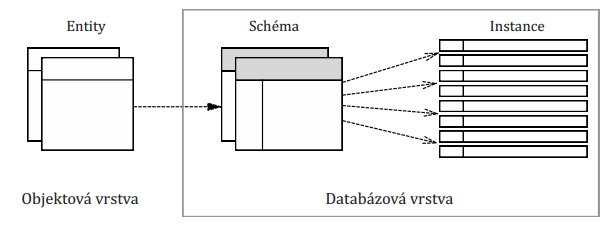
\includegraphics[width=15cm]{figures/framework_structura}
\caption{Rozdělení vrstev softwaru - převzato z \cite{Mazanec}}
\label{fig:mazanma:framework}
\end{center}
\end{figure}
%

\subsection{Metamodely}
Frameworku Migdb je postaven na konceptu MDA \cite{MDA} a pro popsání
jednotlivých vrstev software zavádí pojem metamodel. Metamodel definuje
strukturu popsaných modelů stejně jako model definuje
strukturu dat odpovídajících tomuto modelu.
%
Ve frameworku Migdb jsou popsány dva metamodely - aplikační metamodel a
databázový metamodel. Aplikační metamodel definuje elementy tvořící strukturu
aplikace, množinu aplikačních operací a diff entity použité při rozpoznávání
operací. Databázový metamodel definuje elementy tvořící databázi a operace
aplikovatelné na tyto elementy.\\

Skutečnost, že model A je definován pomocí metamodelu $M_A$, vyjadřuje, že
metamodel $M_A$ popisuje model A a model A je instancí metamodelu $M_A$.

\subsection{Proces transformace modelů}
Proces transformace modelů frameworkem je zobrazen na obrázku
\ref{fig:framework:modified}.
%
\begin{figure}[H]
\begin{center}
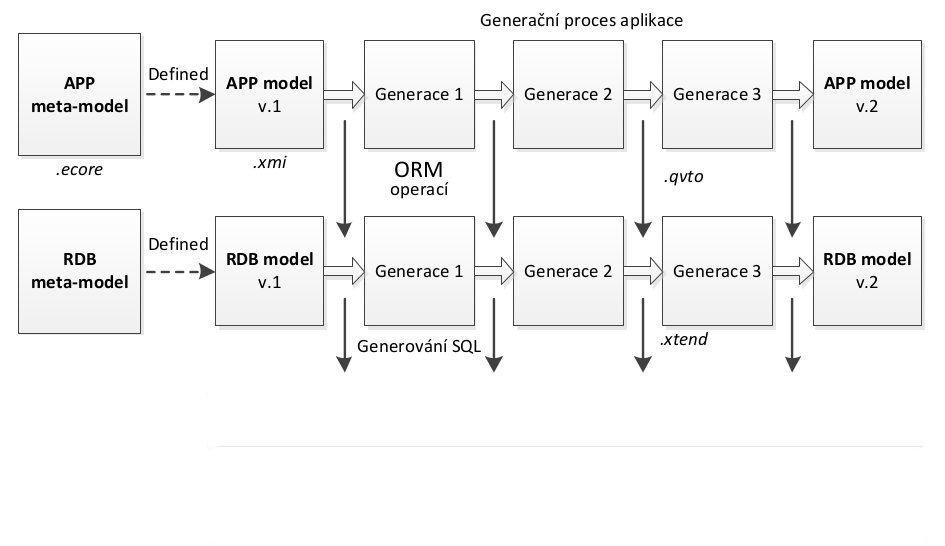
\includegraphics[width=15cm]{figures/framework_structura_tarant_modified}
\caption{Rozdělení vrstev softwaru - převzato z \cite{Tarant_bp} a částečně
upraveno}
\label{fig:framework:modified}
\end{center}
\end{figure}
%
Na obrázku vidíme aplikační a databázový metamodel. Instancemi aplikačního APP
metamodelu jsou jednotlivé aplikační modely. Na vstupní aplikační model v.1 je aplikována
sada aplikačních operací a tento model je transformován do 
výstupního aplikačního modelu v.2. Množinu stavů, kterými aplikační model
prochází před dosáhnutím své výstupní podoby nazýváme generacemi aplikačního
modelu. Procesu změny aplikačního modelu budeme říkat Aplikační Evoluce nebo
Evoluce aplikačního modelu.

Instancemi databázového RDB metamodelu jsou potom jednotlivé RDB modely. Stejně
jako aplikační model je i model databázový postupně transformován. Procesu
vývoje databázového modelu budeme říkat Databázová Evoluce nebo Evoluce
databázového modelu. Stavy, kterými databázový model prochází potom
nazveme generace databázového modelu.

Změny, které se provádějí v aplikaci jsou transformovány na databázové operace
aplikovatelné na RDB model. Databázové operace jsou potom transformovány na SQL
skripty. V původní představě byl do frameworku zapojen i exekutor těchto
skriptů nad databází, ale vzhledem ke znovupoužitelnosti SQL souborů byl z
frameworku vypuštěn.
\FloatBarrier
%
V rámci projektu jsem vytvořil ve své bakalářské práci \cite{Lukes} ORM
transformaci aplikační struktury na databázovou a následné vygenerování SQL
skriptu vytvářející strukturu aplikace. Tento nástroj není ve frameworku použit
při nasazení frameworku, ale byl použit při testování frameworku - viz
kapitola \ref{chapt:testování}. Framework Migdb pracuje oproti původní
sekvenční představě iteračně viz obr. \ref{fig:framework:modified}.
V první iteraci je první aplikační operace aplikována na aplikační model,
transformována do databáze, kde je její obraz (sekvence databázových operací)
aplikován na databázový model. Po provedení první iterace prochází tímto cyklem
druhá operace, potom třetí \ldots
%
\section{Moduly frameworku}
Framework byl od začátku vývoje používán v rámci Eclipse IDE
\cite{Eclipse_ide}. Nad vrstvou aplikační byly vytvořeny 2 moduly. Modul
Operations a modul aplikační evoluce.
 
Modul Operations umožňující napsat vyjádřit vstupní operace pomocí textového
souboru zapsaném v DSL jazyce. Kromě zápisu tento modul transformuje textově
zapsané operace do XMI \cite{XMI} souboru pomocí model to text transformačního
jazyka Xtend \cite{Xtend}. Tento modul je podrobně popsán v
\cite{Mazanec} a není v této práci blíže rozebírán.
 
Modul Aplikační Evoluce definuje pro každou operaci, jaký vliv bude mít
provedení této operace na daný aplikační model a jaké podmínky musí daný
aplikační model splňovat, aby se tato operace dala úspěšně provést. Více v
sekci \ref{sect:app_ops}.
 
Nad databázovou vrstvou je definován modul Databázové Evoluce, který pro
každou databázovou operaci definuje, jaký bude mít tato operace vliv na
databázový model a jaké podmínky musí daný model splňovat, aby se tato operace
mohla úspěšně provést. Více v sekci \ref{db_ops}.\\
 
Spojnici mezi aplikačním a databázovým modulem tvoří dva moduly - modul ORM a
modul ORMo.
 
Modul ORM transformuje model struktury aplikace na model struktury databáze.
Tento modul byl prezentován v mé bakalářské práci \cite{Lukes} a není více v
této diplomové práci rozebírán.
 
Modul ORMo transformuje seznam aplikačních operací na seznam operací
databázových. Tento modul byl popsán v \cite{Jezek} a \cite{Tarant_bp}. Tento
modul tvoří motor celého frameworku a jeho popisu je věnována sekce \ref{ORMo}.\\
 
Výstupem frameworku Migdb není databázový model, ale textový soubor s SQL
příkazy. Textové výstupy vytvářejí dva moduly generátorů kódu. SQL generátor
generuje ze souboru operací výstupní upgrade skript zajišťující samotnou migraci
dat. Schema generator potom generuje ze souboru databázové struktury SQL skript
vytvářející strukturu databáze. Detailnějším popisem implementace těchto modulů
se nebudu v této práci blíže zabývat. Oba dva generátory byly napsány v jazyce
Xtend.\\

Nejnovějším modulem frameworku je modul OpsRecognition. Tento modul se
snaží ze dvou vstupních aplikačních modelů odvodit seznam aplikačních operací.
První vstupní model označíme jako model zdrojový. Druhý vstupní model označíme
jako cílový model. které byly provedeny nad zdrojovým modelem a transformovaly
ho do modelu cílového. Tento modul je samostatným nástrojem a pracuje
nezávisle na ostatních modulech. V rámci tohoto modulu byly definovány dva
algoritmy pro rozpoznávání operací. Tématu rozpoznávání operací je věnována
kapitola \ref{chapt:recognition}.
\\

Moduly Aplikační Evoluce, Databázové Evoluce, ORM, ORMo a OpsRecognition byly
napsány v jazyce QVT Operational (QVTo) \cite{QVTo}.

Za účelem ověření správné funkcionality byl vytvořen projekt Migdb.testing.run,
který je zmíněn v kapitole \ref{chapt:testování}.
%
\section{Aplikační metamodel}
Aplikační metamodel je rozdělen do 3 částí - definice struktury aplikace,
seznam aplikačních operací a seznam rozdílových elementů. Pro každou část je
definován vlastní container, do kterého se ukládají elementy obsažené v této
části. Na obrázku \ref{fig:app_roots} jsou znázorněny kořenové elementy
nynějšího aplikačního modelu - každý aplikační model musí obsahovat nejméně
jeden container - potomka třídy ModelRoot. Aplikační operace jsou popsány v
sekci \ref{sect:app_ops}. Kořenový element Diff je popsán v sekci
\ref{subsect:Diff elementy}.

\begin{figure}[h]
\begin{center}
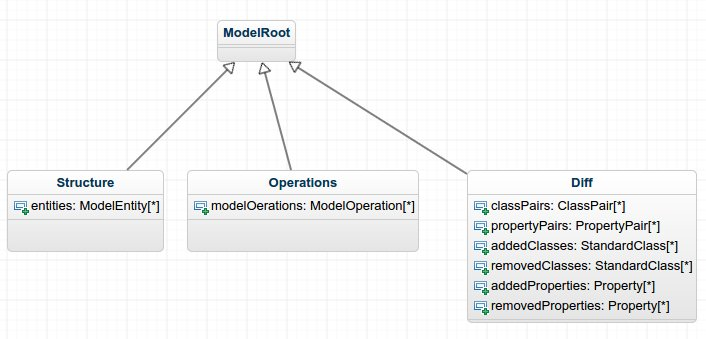
\includegraphics[width=15cm]{figures/app_roots}
\caption{Rootové elementy aplikačního modelu}
\label{fig:app_roots}
\end{center}
\end{figure}
\FloatBarrier

\section{Struktura aplikace}

Struktura aplikace zachycuje vztahy mezi jednotlivými objekty
tvořícími aplikaci. Jednotlivé elementy struktury aplikace jsou obsažené v
kořenovém elementu \textit{Structure}. Na obrázku \ref{fig:app_meta} jsou
zobrazeny elementy patřící do Struktury aplikačního metamodelu.

Struktura aplikačního modelu obsahuje množinu elementů \textit{ModelEntity}.
Každá \textit{ModelEntita} obsahuje svůj identifikátor \textit{name}. Primitivní
typy programovacího jazyka jsou reprezentované elementem \textit{PrimitiveClass}
potomkem \textit{ModelEntity}. První potomek \textit{ModelEntity},
\textit{PrimitiveClass} obsahuje jen \textit{primitiveType}.
Druhým potomkem \textit{ModelEntity} je \textit{StandardClass} a obsahuje
specifikaci svého \textit{inheritancetType}, určující způsob uložení dat.
\textit{StandardClass} dále obsahuje příznak \textit{isAbstract}, referenci na
seznam \textit{Property}, referenci na svou \textit{idProperty} a referenci na
\textit{parent} StandardClass.
Podporujemem pouze jednoduchou dědičnost, proto může mít každá třída maximálně 
jednu rodičovskou třídu. Element \textit{Property} obsahuje svůj \textit{name},
\textit{lowerBound} a \textit{upperBound}, které dohromady určují násobnost
vazby či vymezují vlastnosti primitivní Property. \textit{Property} dále
obsahuje pro kolekce důležité atributy \textit{isUnique} a \textit{isUnique}.
\textit{PrimitiveProperty}, potomek Property, rozšiřuje svou rodičovskou třídu
jen o svůj \textit{type}, který musí být primitivní.
\textit{AssociationProperty}, druhý potomek Property, obsahuje také
\textit{type} [StandardClass], referenci na \textit{oppositteProperty} pro
bidirectional vazby a atribut isOwning, který existuje z implementačních důvodů
více o něm bude zmíněno v kapitole \ref{chapt:dokonceni_projektu}. \\

\begin{figure}[h]
\begin{center}
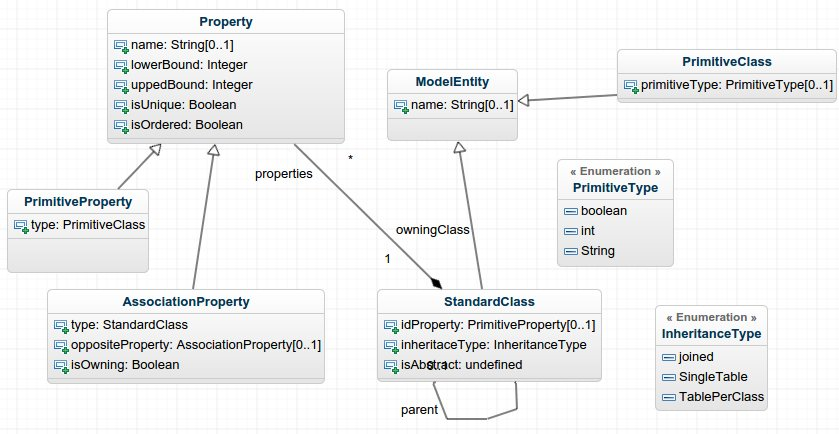
\includegraphics[width=15cm]{figures/app_meta}
\caption{Struktura aplikačního metamodelu}
\label{fig:app_meta}
\end{center}
\end{figure}
\FloatBarrier

\section{Struktura databáze}
 Databázový metamodel od počátku vývoje definuje elementy nutné k specifikaci
 struktury databáze a databázové operace. Námi používanou databází je databáze
 PostgreSql, databázový metamodel je vytvořen na základě této
 databáze a může se mírně odklánět od jiných relačních databází.
 Základním databázovým konstruktem je \textit{Schema}, které je jednoznačně
 identifikované svým \textit{name}, obsahuje sezname tabulek a seznam
 sekvencí.
 \textit{Sequence} je databázový element potřebný k postupnému
 generování čísel, je identifikovaná pomocí svého \textit{name} a musí
 obsahovat své \textit{startValue}.
 Každá \textit{Table} má své \textit{name}, obsahuje seznam \textit{Column} a
 seznam \textit{TableConstraint}. Každý \textit{Column} má své \textit{jméno},
 atribut \textit{nillable}, který povoluje či zakazuje NULL hodnoty v tomto sloupci,
 \textit{type} [PrimitiveType] a odkaz na vlastnickou tabulku
 \textit{owningTable}.

Potomci \textit{TableConstraint} jsou jednotlivé IO a mají společné
\textit{name} zpřístupňující daný TableConstraint.  TableConstraint
\textit{Unique} obsahuje seznam unikátních sloupců \textit{uniqueColumns} a
odkaz na vlastnickou tabulku \textit{ownintTable}.
Ačkoliv je v databázi možné mít vícesloupcový primární klíč, omezili jsme si
\textit{PrimaryKey} tak, aby ho bylo možné definovat jen nad jedním sloupcem
\textit{constrainedColumn}, protože již od začátku vývoje bylo zřejmé, že
v našem frameworku budeme pracovat jen s umělými jednosloupcovými klíči.
\textit{ForeignKey} je poslední TableConstraint a podobně jako PrimaryKey má
omezen počet sloupců tvořící cizí klíč na jeden \textit{constrainedColumn} a
obsahuje také odkaz na referencovanou tabulku \textit{targetTable}. Na obr.
\ref{fig:rdb_str} je zobrazen aktuální databázový metamodel.


\begin{figure}[H]
\begin{center}
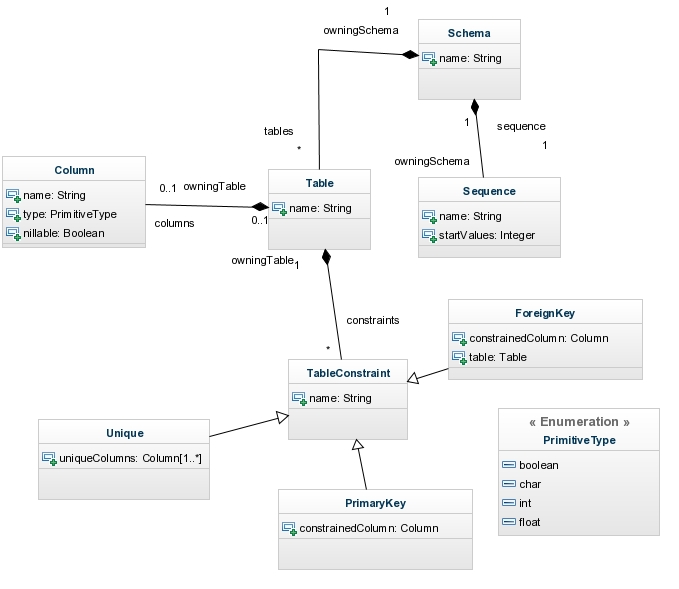
\includegraphics[width=15cm]{figures/rdb_structure}
\caption{Struktura databázového metamodelu}
\label{fig:rdb_str}
\end{center}
\end{figure}
%
\FloatBarrier

%\section{Relační model}
%Relační model je dle \cite{DBS_02} formální abstrakce
%využívající relaci jakožto jediný konstrukt. Relace je uspořádaná n-tice
%souvislých dat R(A1:D1, A2:D2, \ldots An:Dn), přičemž "R" je název relace, Ai
%jsou názvy atributů a Di jsou k nim přidružené typy. K zajištění konzistence
%jsou v SŘDB používána Integritní omezení (IO). IO jsou dle \cite{DBS2_02}
% tvrzení vymezující korektnost DB, stupeň souladu datového obrazu s předlohou (jaká data
%v databází mohou být a jaká již ne).


%Relační algebra definuje pomocí relací a integritních omezení strukturu
%databáze. Dotazovacím aparátem pro data definovaná pomocí relační algebry je
%relační algebra. Relační algebra využívá operátorů $\bigcup$ (sjednocení),
%$\bigcap$ (průnik), $\setminus$ (množinový rozdíl), $\times$ (kartézský
%součin), selekce značená R($\varphi $) = \{ u | u $\in$ R a  $\varphi(u)$\} a
%projekce značená R[C] = { u[C] | u $\in$ R} a operace přirozené spojení T(C) =
%R * S =\{u | u[A] $\in$ R a u[B] $\in$ S\}.
%\cite{DBS_02} dále definuje relačně úplný jazyk jako takový, který
%umožňuje realizovat relační algebru. Takovým jazykem je například jazyk SQL 
%(Structured Query Language). Relační databáze implementuje relaci tabulkou,
% její atributy Ai jednotlivými sloupci s typy Di. V dotazovacím jazyce SQL nahrazuje
%projekci R[a1, \ldots , an] operací SELECT a1, \ldots an FROM R, operaci
%selekce R[ a = 1] klauzulí where v dotaze select  SELECT * FROM R WHERE a = 1; 

\section{Operace nad aplikačním modelem} \label{sect:app_ops}
Operace nad aplikačním modelu definují možné transformace, které je možné
provést aplikačním modelem. Každá aplikační operace má definované dvě metody.
První metodou je metoda se signaturou boolean isValid(Structure structure),
která pro danou aplikační strukturu zjistí, jestli je daná operace proveditelná
nad touto strukturou, a vrátí tuto informaci ve své návratové hodnotě. Druhá
metoda se signaturou void apply(Structure structure) aplikuje operaci na danou
strukturu, tj. pozmění elementy v ní obsažené.

\subsection{Seznam aplikačních operací}

Operace jsou uvedeny v následujícím seznamu. Pro každou operaci jsou v seznamu
uvedeny její validační podmínky a důsledky změny aplikace na model struktury.
Validační podmínky určují, kdy by měla metoda isValid pro danou strukturu vracet
true.

Kromě regulérních operací, které může vytvořit uživatel jsou v tabulce uvedeny i
virtuální operace DistributeProperty, MergeProperty a operace ExportProperty.
Virtuální operace nemůže vytvořit uživatel, jsou používány jako pomocné v
implementaci složitějších operací a manipulují s Property v rámci dědičné
hierarchie tříd. Tyto operace mohou narozdíl od nevirtuálních operací být
aplikovány na model, který je z nějakého hlediska nevalidní a nemají
definovanou operaci isValid.
Například operace MergeProperty počítá s hierarchií s kolizní property v třídě
předka a potomka. Hlavním přínosem virtuálních operací je zabránění duplikace v
definici ORMo mapování a zjednodušení kódu.

\newcounter{ListCitac}
\begin{list}{Operace \Roman{ListCitac}:}{\usecounter{ListCitac}}
  \item AddStandardClass(name, isAbstract, inHeritanceType)
  \begin{itemize}
    \item Validační podmínky - neexistuje třída s jménem nově vznikající
    \item Operace vytvoří novou třídu a její id odvozené z názvu třídy
  \end{itemize}
  \item RenameEntity(name, newName)
  \begin{itemize}
    \item Validační podmínky - existuje třída s původním jménem, neexistuje
    třída s novým jménem
    \item Operace změní název třídy na nový
  \end{itemize}
  \item SetAbstract(name, isAbstract)
  \begin{itemize}
    \item Validační podmínky - existuje třída s daným jménem
    \item Operace nastaví třídě atribut abstract na danou hodnotu    
  \end{itemize}
  \item RemoveEntity(name)
  \begin{itemize}
    \item Validační podmínky - existuje třída s daným jménem, neexistuje
    asociační property odkazující typem na tuto třídu, třída neobsahuje žádné
    property, neexistuje pro tuto třídu žádný potomek
    \item Operace odstraní entitu (standardní třídu) z modelu
  \end{itemize}
  \item AddProperty(owningClassName, name, typeName, lowerBound, upperBound,
  isOrdered, isUnique) 
  \begin{itemize}
    \item Validační podmínky - zadané bounds jsou validní, v hierarchii
    dědičnosti neexistuje kolizní property se stejným jménem, existuje
    ModelEntity s názvem shodným s typeName
    \item  Operace vytvoří v dané třídě novou property se zadanou horní mezí,
    dolní mezí, typem, seřaditelností a unikátností
  \end{itemize}
  \item RenameProperty(owningClassName, name, newName)
  \begin{itemize}
    \item Validační podmínky - existuje přejmenovaná property v dané třídě,
    nexistuje property s jménem shodným s newName v dané třídě 
    \item  Operace změní název property v dané třídě ze starého na nový
  \end{itemize}
  \item RemoveProperty(owningClassName, name)
  \begin{itemize}
    \item Validační podmínky - musí exitovat vlastnická třída property a v ní
    odstraňovaná property
    \item  Operace odstraní property z dané třídy
  \end{itemize}
  \item SetBounds(upperBound, lowerBound)
  \begin{itemize}
    \item Validační podmínky - bounds musí být validní a musí existovat daná
    trída a property
    \item  Operace nastaví horní a dolní mez property na nové hodnoty
  \end{itemize}
  \item SetOrdered(owningClassName, name, isOrdered)
  \begin{itemize}
    \item Validační podmínky - musí existovat daná trída a property
    \item  Operace nastaví property atribut isOrdered na odpovídající hodnotu
  \end{itemize}
  \item SetUnique(owningClassName, name, isUnique)
  \begin{itemize}
    \item Validační podmínky - musí existovat daná třída a property
    \item  Operace nastaví property atribut isUnique na odpovídající hodnotu
  \end{itemize}
  \item AddParent(className, parentClassName)
  \begin{itemize}
    \item Validační podmínky - musí existovat rodičovská třída a třída potomka,
    třída potomka nesmí mít nastaveného rodiče
    \item Operace nastaví třídě předka a přesune namerguje (aplikuje virtuální
    operaci MergeProperty) kolizní atributy do rodičovské třídy
  \end{itemize}
  \item RemoveParent(className, parentClassName)
  \begin{itemize}
    \item Validační podmínky - musí existovat třída s name className a mít
    nastavenou hodnotu parent != NULL
    \item Operace odstraní třídě s name rovným className rodičovskou třídu a
    použije virtuální operaci DistributeProperty na property z rodičovské třídy
    do třídy původního potomka
  \end{itemize}
  \item ExtractClass(sourceClassName, extractClassName,
  associationPropertyName, oppositePropertyName, propertyNames)
  \begin{itemize}
    \item Validační podmínky - musí existovat zdrojová třída, neexistuje
    property s jménem linku na nově vzniklou třídu, existují exportované property
    \item Operace vytvoří novou třídu, kterou napojí na původní třídu přes
    asociační property associationPropertyName, exportuje(využije virtuální
    operaci export property) do nově vzniklé třídy vyjmenované property
  \end{itemize}
  \item InlineClass(targetClassName, associationPropertyName)
  \begin{itemize}
    \item Validační podmínky - musí existovat cílová třída a
    musí existovat asociační property s jménem associationPropertyName typu
    Inlinované třídy, která má upper bound 1
    \item Operace exportuje (aplikuje virtuální operaci exportProperty)
    na všechny property z inlinované třídy do cílové třídy přes specifikovanou
    unidirectional asociaci
  \end{itemize}
  \item ChangeUniToBidir(className, associationPropertyName, oppositePropertyName)
  \begin{itemize}
    \item Validační podmínky - v dané třídě musí existovat asociační property
    s daným jménem a nesmí mít nastavenou opposite property 
    \item Operace vytvoří nový zpětný link s oppositePropertyName k property
    targetClassName a nastaví správně data do opepositePropertyName
  \end{itemize}
  \item ChangeBiToUnidir(className, associationPropertyName)
  \begin{itemize}
    \item Validační podmínky - v dané třídě musí existovat asociační property
    s daným jménem a musí mít nastavenou opposite property
    \item Operace odstraní opoziční property
  \end{itemize}
  \item CollapseHierarchy(superClassName, subClassName, isIntoSub)
  \begin{itemize}
    \item Validační podmínky - musí existovat subclass a superclass, subclass
    musí mít nastavenou superclass jako parenta
    \item Operace exportuje (aplikuje virtuální operaci ExportProperty)
    všechny property z jedné třídy do jejího předka a třídy spojí, upraví
    dědičné vazby
  \end{itemize}
  \item ExtractSubClass(sourceClassName, extractedClassName, extractedPropertyNames)
  \begin{itemize}
    \item Validační podmínky - musí existovat třída s name sourceClassName a
    nesmí existovat třída s jménem extractedClassName, v třídě sourceClass musí
    existovat property s názvy z kolekce extractedPropertyNames
    \item Operace vytvoří třídě nového potomka a
    exportuje (aplikuje virtuální operaci export property) do něj vyjmenované
    property
  \end{itemize}
  \item ExtractSuperClass(sourceClassesName, extractParentName, propertyNames)
  \begin{itemize}
    \item Validační podmínky - musí existovat třída s name sourceClassName a
    nesmí existovat třída s jménem extractedParentName, v třídě sourceClass musí
    existovat property s názvy z kolekce propertyNames
    \item Operace vytvoří třídě nového předka a přesune do něj vyjmenované
    property, pokud měla původní třída předka nastaví tohoto předka rodičem 
    nově vzniklé třídě
  \end{itemize}
  \item PullUpProperties(childClassName, pulledPropertiesNames)
  \begin{itemize}
    \item Validační podmínky - musí existovat childClass a mít nastavenou
    rodičovskou třídu, v třídě potomka musí existovat properties z kolekce
    pulledPropertiesNames, v okolních subhierarchiích nesmí existovat properties
    z této kolekce
    \item Operace exportuje (aplikuje virtuální operaci export property)
    property do rodičovské třídy
  \end{itemize}
  \item PushDownProperties(childClassName, pushedPropertiesNames)
  \begin{itemize}
    \item Validační podmínky - musí existovat class s childClassName a mít
    nastavenu parentClass, v třídě potomka musí existovat properties z kolekce
    pushedPropertiesNames
    \item Operace exportuje(aplikuje virtuální operaci export property) 
   vyjmenované property do třídy potomka a přesune JEN data potomka
  \end{itemize}
  \item ExportProperty(exportedPropertyName, className)
  \begin{itemize}
    \item virtuální operace
    \item Operace přesune property a data v ní obsažená v rámci hierarchie do
    cílové třídy
  \end{itemize}
  \item DistributeProperty(distributedPropertyName, className)
  \begin{itemize}
    \item virtuální operace
    \item Operace zduplikuje strukturu v rámci hierarchie dané property do
    cílové třídy a přesune data přiřazená této třídě
  \end{itemize}
  \item MergeProperty(mergedPropertyName, className)
  \begin{itemize}
    \item virtuální operace
    \item Operace přesune data zdrojové property do cílové property a smaže
    strukturu původní property
  \end{itemize}
\end{list}

\subsection {Rozdělení aplikačních operací} 

Operace nad aplikačním modelem je možné dělit podle dvou kritérií - 1. nad jakým
typem modelové entity pracují, 2. jaký je charakter/význam pro tito entity daná
operace má. Operace byly rozděleny podle obou kritérií spíše formálně. Všechny operace
jsou potomkem generické operace ModelOperation. Rozdělení podle druhého kritéria
vzniklo až po přidání funkcionality rozpoznávání operací.

První kritérium dělí aplikační operace na operace pracující s třídami a operace
pracující pouze s properties daných tříd. Příkladem operací pracujících s
třídami jsou operace AddStandardClass, AddParent a RemoveEntity. Příkladem
operací pracujících s properties jsou operace AddProperty, RemoveProperty, SetAbstract.

Podle druhého kritéria je možné rozdělit operace nad aplikačním modelem do 5
skupin - konstruktivní, destruktivní, expanzivní, reduktivní a modifikační operace.
Konstruktivní operace jsou takové, které po své aplikaci vytvoří 1 novou entitu
ve výsledném modelu, která nemá žádné vazby na jiné entity. Příklady aditivní
operace je operace AddClass. 

Destruktivní operace je opak konstruktivní, ve vstupním modelu existuje entita a
ta je aplikaci destruktivní operace odstraněna. Příkladem destruktivní operace
je operace RemoveProperty.

Operace expanzivní přídává do výstupního modelu jednu entitu, čímž se
podobá operaci konstruktivní, nicméně zároveň je vázána na jinou entitu
stejného typu a mění její obsah. Příkladem expanzivní operace je
ExtractClass.

Reduktivní operace entitu z vstupního modelu odstraní a zároveň entitě, která
je pro operaci řídící změní obsah. Příkladem této operace je InlineClass.
Reduktivní operace jsou inverzní k operacím expanzivním.\\

\section{Databázové operace} \label{db_ops}

Databázové operace popisují transformace, které mohou být provedeny nad
databázovým modelem v průběhu Evoluce databázového modelu. Každá databázová
operace má definovány dvě metody boolean isValid(Structure structure) a
void apply(Structure structure). Metody mají stejný význam jako metody
stejnojmenných aplikačních operací, jen pracují s databázovým modelem místo
aplikačního. Metoda isValid(Structure structure) určuje, jestli je operace
aplikovatelná na daný model databázové struktury. Metoda apply potom definuje
důsledky, které má aplikace operace na daný databázový model.

Databázové operace reprezentují změny proveditelné na úrovni databáze. Mělo by z
nich být možné generovat SQL kód jednoduchou Model-to-text transformací
zajišťovanou modulem Generator.xtend.

Seznam operací s jejich validačními podmínkami a důsledky jejich aplikakace je
uveden v následujícím seznamu:

\newcounter{ListCitac2}
\begin{list}{Operace \Roman{ListCitac2}:}{\usecounter{ListCitac2}} 
  \item AddSchema(name)
  \begin{itemize}
    \item Vytvoří nové schéma s zadaným jménem
    \item Nesmí existovat schéma s zadaným
    jménem
  \end{itemize}
  \item AddSequence(owningSchemaName, name, startValue)
  \begin{itemize}
    \item Vytvoří v cílovém schématu sekvenci s zadanou startovní hodnotou
    \item Musí existovat schéma, do kterého se vkládá, v něm nesmí existovat
    sequence s jménem name
  \end{itemize}
  
  \item AddTable(owningSchemaName, name)
  \begin{itemize}
    \item V daném schématu vytvoří tabulku, id sloupec této tabulky a primární
    klíč odvozený z jména tabulky
    \item Musí existovat dané schéma, v
    němž nesmí existovat tabulka s jménem name
  \end{itemize}
  
  \item AddColumn(owningSchemaName, owningTableName, name, type)
  \begin{itemize}
    \item Vytvoří v daném schématu a tabulce column s zadaným primitivním typem
    \item Musí existovat dané schéma, tabulka a v dané lokaci nesmí existovat
    daný sloupec
  \end{itemize}
  
  \item AddPrimaryKey(owningSchemaName, owningTableName,
  constrainedColumnName, name)
  \begin{itemize}
    \item Vytvoří v daném schématu a tabulce nad constrainedColumn Primární klíč
    s daným jménem
    \item Musí existovat dané schéma, daná tabulka, daná column, nesmí existovat
    constraint s daným jménem
  \end{itemize}

  \item AddForeignKey(owningSchemaName, owningTableName, constrainedColumnName,
  name, targetTableName)
  \begin{itemize}
    \item Vytvoří v daném schématu a tabulce cizí klíč s daným jménem, který
    referencuje IdColumn cílové tabulky
    \item Musí existovat dané schéma, daná tabulka, daná column, nesmí existovat
    constraint s daným jménem, musí existovat targetTable
  \end{itemize}
  
  \item AddUnique(owningSchemaName, owningTableName,
  constrainedColumnNames, name)
  \begin{itemize}
    \item Vytvoří v daném schématu a tabulce unique constraint s daným jménem
    nad zadanými sloupci
    \item Musí existovat dané schéma, musí existovat daná tabulka, musí
    existovat dané constrainované sloupce, nesmí existovat constraint s jménem
    name
  \end{itemize}

  \item AddNotNull(owningSchemaName, owningTableName, constrainedColumnName)
  \begin{itemize}
    \item Nastaví v daném schématu a tabulce cílové property hodnotu notNull na
    true
    \item Musí existovat dané schéma, daná tabulka, daná column
  \end{itemize}

  \item RemoveNotNull(owningSchemaName, owningTableName, constrainedColumnName)
  \begin{itemize}
    \item Nastaví v daném schématu a tabulce cílové property hodnotu notNull na
    false
    \item Musí existovat dané schéma, daná tabulka, daná column
  \end{itemize}

  \item RenameTable(owningSchemaName, name, newName)
  \begin{itemize}
    \item Změní cílové tabulce jméno na nové
    \item Musí existovat dané schéma, daná tabulka, nesmí existovat tabulka s
    novým jménem
  \end{itemize}

  \item RenameColumn(owningSchemaName, owningTableName, name, newName)
  \begin{itemize}
    \item Přenastaví v daném schématu a tabulce jméno z name na hodnotu newName
    \item  Musí existovat dané schéma, daná tabulka, daná column
  \end{itemize}

  \item RemoveTable(owningSchemaName, name)
  \begin{itemize}
    \item Odstraní z daného schematu tabulku s jménem name
    \item Musí existovat dané schéma, daná tabulka
  \end{itemize}

  \item RemoveColumn(owningSchemaName, owningTableName, name)
  \begin{itemize}
    \item Odstraní v daném schématu a tabulce column s jménem name
    \item Musí existovat schéma s name owningSchemaName, tabulka s name
    owningTableName, sloupec s name rovým name. Sloupec nesmí obsahovat
    constraint PrimaryKey, ForeignKey ani Unique
  \end{itemize}

  \item RemoveConstraint(owningSchemaName, owningTableName, name)
  \begin{itemize}
    \item Přenastaví v daném schématu a tabulce column s jménem name
    \item  Musí existovat dané schéma, tabulka a column
  \end{itemize}

  \item RemoveSequence(owningSchemaName, name)
  \begin{itemize}
    \item Odstraní v daném schématu sequence s jménem name
    \item Musí existovat dané schéma a daná sequence
  \end{itemize}

  \item UpdateRows(owningSchemaName, sourceTableName,
  sourceColumnName, targetTableName, targetColumnName,
  selectionWhereCondition, safeWhereCondition)
  \begin{itemize}
    \item v daném schématu updatuje hodnoty z tabulky sourceTable hodnoty z
    sourceColumns a nastaví je do taragetColumns tabulky targetTable pro
    instance splňující selectionWhereCondition, pozn. aby nebyly nullovány
    hodnoty, pro které nebyly vybrány hodnoty z sourceTable byla přidána
    safeWhereCondition
    \item Musí existovat dané schéma, v něm sourceTable, v ní sourceColumn, v
    dále musí v schématu existovat targetTable, v ní targetColumn, sourceColumn
    musí mít stejný typ jako targetColumn
  \end{itemize}

  \item NillRows(owningSchemaName, tableName, columnName, whereCondition)
  \begin{itemize}
    \item Nastraví sloupci v daném schematu a tabulce hodnoty null instancím
    splňující whereCondition
    \item Musí existovat dané schéma, daná tabulka, daná column
  \end{itemize}

  \item InsertRows(owningSchemaName, sourceTableName, sourceColumnName,
  targetTableName, targetColumnName, whereCondition)
  \begin{itemize}
    \item v daném schématu zkopíruje z tabulky sourceTable hodnoty z
    sloupce sourceColumns instance splňující whereCondition a vloží je do
    taragetColumns tabulky targetTable    
    \item Musí existovat schéma s name owningSchemaName, v něm table
    identifikovaná sourceTableName, v ní column identifikovaná sourceColumnName,
    Ve schématu musí existovat table identifikovaná targetTableName, v ní
    column identifikovaná targetColumnName. SourceColumn musí mít stejný typ
    jako targetColumn
  \end{itemize}

  \item DeleteRows(owningSchemaName, tableName, whereCondition)
  \begin{itemize}
    \item Operace smaže z daného schematu, instance z dané table
    splňující whereCondition
    \item Musí existovat dané schéma, v něm daná table
  \end{itemize}

\end{list}

\section{QVTo}
QVTo je imperativní jazyk, který je součástí standardu QVT definovaným
konsorciem Object Management Group (OMG) viz. \cite{OMG}. Součástí QVT je
jazyk OCL (Object Constraint Language) \cite{OCL}. Pomocí tohoto jazyka je možné
definovat model to model transformaci.

Základními konstrukty jazyka jsou mapping, helper a query. Mapping je konstrukt
měníci pomocí nějakých pravidel vstupní element na výstupní. Query je
dotazovací konstrukt, který získá potřebnou výstupní informaci z daného
elementu. Helper je konstrukt, který může narozdíl od query měnit objekt, nad
kterým byl helper vyvolán.

Na následující ukázce vidíme ukázkový HelloWorld příklad QVTo kódu převzatý z
\cite{QVTO_Example}


\begin{verbatim}
modeltype ABC uses ABC('http:///ABC.ecore');

transformation HelloWorld(in source:ABC, out target:ABC);

main() {
   source.rootObjects()[Root]->map Root2Root();
}

mapping Root :: Root2Root() : Root {
   element += self.element[A]->map A2B();
}

mapping A :: A2B() : B
 when {
      self.id > 0
 }
   {
      result.id := self.id;
      result.b := self.a + " World!";
   }
\end{verbatim}


Na začátku každého .qvto souboru můžeme importovat potřebné knihovny
pomocí klíčového slova import, čehož v ukázce nebylo zapotřebí. Následně
deklarujeme typy modelů, které bude naše transformace používat pomocí klíčového
slova modeltype. Metamodel ABC použitý v tomto příkladě je zobrazen na obrázku
\ref{fig:qvto_example}. 

V metamodelu ABC je každý kořenový element složen z 0\ldots n entit Element.
Entita Element má své Id. Existují tři potomci entity Element, třídy A, B, C.
Každý potomek entity Element obsahuje atribut typu řetězec, který má jméno
shodné s názvem třídy. Každá Entita element může být obsahovat 0\ldots n
subelementů typu Element.

\begin{figure}[h]
\begin{center}
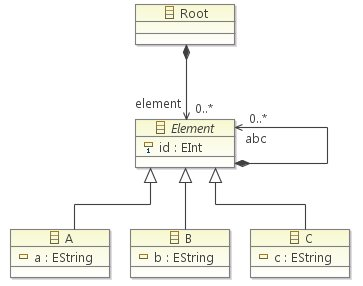
\includegraphics[width=7cm]{figures/qvto_example_metamodel}
\caption{ABC metamodel převzatý z \cite{QVTO_Example}}
\label{fig:qvto_example}
\end{center}
\end{figure}
\FloatBarrier

Řádek \textit{transformation HelloWorld(in source:ABC, out target:ABC);} nám
definuje hlavičku transformace. Název transformace je HelloWorld a transformace
mapuje jeden vstupní model \textit{source} typu ABC na jeden výstupní model
\textit{target} typu ABC. Kromě vstupních a výstupních elementů mohou být v
transformaci modely vstupně-výstupní označené klíčovým slovem inout.

Vstupním bodem každé transformace je metoda main. Ukázkový příklad v metodě main
přistupuje pomocí \textit{source.rootObjects()} k kořenovým elementům source
modelu, vybírá z nich pomocí \uv{[Root]} všechny elementy typu Root.
\textit{source.rootObjects()[Root]} je ekvivalentní s ocl selectem
\textit{source.rootObjects()->select(e |
e.oclIsTypeOf(Structure)).oclAsType(Structure)}.
Transformace volá nad vybranou kolekcí elementů mapování Root2Root pomocí
\textit{->map Root2Root()}. 

Mapování Root2Root s hlavičkou \textit{mapping Root:: Root2Root() : Root}
mapuje Element typu Root na jiný Element typu Root. V těle metody je vybrán
každý element typu A z kolekce elementů vstupního elementu Root viz
\textit{self.elements[A]} a výsledek volání mapování A2B() je přidán do
kolekce elements výstupní entity Root.

Mapování A2B() mapuje entity typu A na elementy typu B. Kódem v bloku when
je určuna doplňující podmínka, mapovat se budou jen entity typu A s id > 0.
Mapování nastaví výsledné entitě id vstupní entity a rozšíří text uložený v
entitě o řetězec \textit{World!}. 

Ukázkový kód bude tedy transformovat vstupní model 
\begin{verbatim}
 ROOT:
   A: id=1, A=”Hello”
   A: id=-1, A=”World”
   C: id=1, C=”Something”
\end{verbatim}

Na výstupní model
\begin{verbatim}
   A: id=1, A=”Hello World!”
\end{verbatim}

\subsection{Ukázka kódu Migdb}
Jak již bylo řečeno v předchozí sekci, je možné kromě mapování definovat
dotazovací konstrukt query a modifikační konstrukt helper. Oba konstrukty jsou
si velmi podobné, jejich jedinou odlišností je, že query nesmí modifikovat
objekt, nad kterým je voláno a helper může. V následujícím kódu je ukázáno
validační query pro zjištění splnitelnosti validačních podmínek operace
AddTable. Query isValid převolává dvě helpery. V helperu checkExistSchema
vidíme kontrolu a případné zalogování chyby při nenalezení schématu, Není tedy
možné vracet obrácenou hodnotu volání pokud chceme zjistit, že daná validační
podmínka neplatí, protože by tímto voláním byla zalogována chyba.

\begin{verbatim}
query RDB::ops::AddTable::isValid(structure : RDB::Structure, 
  inout errorLog : ErrorLog, operationIndex : Integer) : Boolean {
    var existSchema : Boolean := checkExistSchema(
                                        self.owningSchemaName, 
                                        structure, 
                                        errorLog, 
                                        operationIndex, 
                                        getEvolutionRdbTransformationId());
    var notExistTable : Boolean := checkNotExistTable(
                                        self.owningSchemaName, 
                                        self.name, 
                                        structure, 
                                        errorLog, 
                                        operationIndex, 
                                        getEvolutionRdbTransformationId());
    return existSchema and notExistTable;
}

helper checkExistSchema(schemaName : String, structure : Structure, 
  inout errorLog : ErrorLog, operationIndex : Integer, 
  transformationId : String) : Boolean{ 
    var existSchema : Boolean := structure.containsSchema(schemaName);
    if(not existSchema)then{
        var errorMessage : String := "Schema " + schemaName + " doesn't exist";
        errorLog.errors += _evolutionError(
                                          operationIndex, 
                                          errorMessage,
                                          transformationId); 
    }endif;
    return existSchema;        
}

\end{verbatim}

\section{ORMo (ORM operací)}\label{ORMo}

ORMo mapování je transformace, která mapuje elementy z dómény aplikačních
operací na elementy z domény operací databázových. Toto mapování mapuje 1
aplikační operaci na 0 až N operací databázových. Většinou je aplikační
operace namapována na nejméně 1 databázovou operaci. Výjimkou je operace
SetAbstract pro případ v případě, že měníme abstraktní třídu na neabstraktní.

Ačkoliv ORM transformace vstupního aplikačního modelu funguje se všemi
inheritanceTypy bylo nutné zjednodušit aplikační model tak, aby byla
transformace ORMo implementovatelná, proto jsme v rámci týmu Migdb rozhodli o
redukci počtu inheritanceTypů na jeden - nejvhodnější typ je joined, který je
nejvíce používaným.

\begin{list}{Operace \Roman{ListCitac}:}{\usecounter{ListCitac}}
  \item AddStandardClass(name, isAbstract, inHeritanceType)
  \begin{itemize}
    \item Vytvoří tabulku, id sloupec této tabulky a primární klíč
  \end{itemize}
  
  \item AddProperty(owningClassName, name, typeName, lowerBound, upperBound,
  isOrdered, isUnique)
  \begin{description}
    \item[Primitivní typ a UpperBoubd = 1] operace přidá do vlastnické tabulky
    sloupec pro primitivní property
    \item[Primitivní typ a UpperBound != 1] operace přidá do modelu tabulku,
    která je obrazem kolekce, do této tabulky přidá datový sloupec, referenční
    sloupec a ForeignKey referencující tabulku, která je obrazem vlastnické třídy
    \item[Neprimitivní typ a UpperBound = 1] operace přidá do tabulky, která je
    obrazem vlastnické třídy property a ForeignKey odkazující na tabulku, která
    je obrazem třídy typu přidávané property
    \item[Neprimitivní typ a UpperBound != 1] operace vytvoří vazební tabulku
    pro neprimitivní property, vloží do ní referenční sloupce na tabulku, která je
    obrazem vlastnické třídy, a tabulku, která je obrazem třídy typu. Nad
    vazební tabulkou vytvoří cizí klíče na tabulku, která je
    obrazem vlastnické třídy, a cizí klíč na tabulku, která je obrazem třídy
    typu
  \end{description}
  
  \item RenameEntity(owningClassName, name, newName)
  \begin{itemize}
    \item Operace změní název tabulky na nový, odstraní a vytvoří PK s
novým jménem, odstraní všechny ForeignKey referencující obraz vlastnické
třídy a vytvoří nové ForeignKey s pozměněným jménem
  \end{itemize}
  
  \item SetAbstract(name, isAbstract)
  \begin{description}
    \item[isAbstract = true] maže data, která náleží pouze dané třídě
    \item[isAbstract = false] mapuje na prázdnou množinu operací
  \end{description}
  
  \item RemoveEntity(name)
  \begin{itemize}
    \item operace smaže primární klíč, id property a tabulka
odpovídající dané třídě
  \end{itemize}
  
  \item RenameProperty(owningClassName, name, newName)
  \begin{description}
  \item[primitivní typ a UpperBound = 1] přejmenuje property v
  tabulce, která je obrazem vlastnické třídy property
  \item[primitivní typ a UpperBound != 1] přejmenuje datový sloupec, odstraní
  a vytvoří ForeignKey s novým jménem referencujícím třídu, která je obraz
  vlastnické třídu property a přejmenuje tabulku obrazu kolekce
  \item[neprimititní typ a UpperBound = 1] přejmenuje sloupec v
  tabulce, která je obrazem vlastnické třídy property, odstraní a vytvoří
  ForeignKey referující tabulku, která je obrazem třídy typu
  \item[neprimitivní typ a UpperBound != 1] přejmenuje vazební tabulku s
  referenčními sloupci na tabulku, která je obrazem třídy vlastníka property a
  tabulku, který je obrazem třídy typu asociace, odstraní a vytvoří ForeignKey s
  novými jmény na obraz třídy vlastníka property a obraz třídy typu
  \end{description}

  \item RemoveProperty(owningClassName, name)
  \begin{description}
  	\item[primitivní typ a UB = 1] odstraní sloupec z dané tabulky
	\item[primitivní typ a UB != 1] odstraní referenci na vlastnickou tabulku,
	sloupec z tabulky dané kolekce, datový sloupec a smaže kolekční tabulku
	\item[neprimitivní typ a UB = 1] odstraní referenci na tabulku vlastníka a
	referenční sloupec
	\item[neprimitivní typ a UB != 1] odstraní reference na vlastnickou tabulku a
	tabulku typu, datový sloupec a sloupec typu a smaže vazební tabulku
  \end{description}

   %\item SetBounds()
   %\begin{itemize}
   %\itemNEIMPLEMENTOVÁNO \\
	%\end{itemize}

  \item SetOrdered(owningClassName, name, isOrdered)
  \begin{description}
  	\item[isOrdered = true] přidá sloupec ordering, přenastaví data a vytvoří
  	unikátní constraint přes typový, referenční a orgering sloupec
	\item[isOrdered = false] smaže ordering unique constraint a ordering sloupec 
  \end{description}

  \item SetUnique(owningClassName, name, isUnique)
  \begin{description}
  	\item[isUnique = true] vytvoří unikátní constraint přes typový a referenční
  	sloupec
	\item[isUnique = false] smaže unique constraint
  \end{description}
  
  \item AddParent(className, parentClassName)
  \begin{itemize}
    \item Aplikuje obraz operace MergeProperty na všechny kolizní property,
	přidá cizí klíč na rodičovskou třídu
  \end{itemize}

  \item RemoveParent(className)
  \begin{itemize}
    \item aplikuje obraz operace DistrubuteProperty na všechny property
	rodičovské třídy, odstraní cizí klíč, smaže data třídy potomka z tabulky
	rodiče
  \end{itemize}

  \item ExtractClass(sourceClassName, extractClassName, associationPropertyName,
  oppositePropertyName, propertyNames)
  \begin{itemize}
    \item vytvoří novou sekvenci, vytvoří novou
    tabulku. Do této tabulky vytvoří nové sloupce extrahovaných properties a 
    sloupec pro opposite referenci na zdrojovou tabulku. Aplikuje obraz operací
    exportProperty pro každou exportovanou property, vytvoří sloupec
    referencující nově vzniklou tabulku, updatuje mu hodnoty, smaže
    vygenerovanou sekvenci
  \end{itemize}
  
  \item InlineClass(targetClassName, associationPropertyName)
  \begin{itemize}
    \item aplikuje obraz operací exportProperty, smaže association column a
	Inlinovanou tabulku
  \end{itemize}

%\item ChangeUniToBidir & pro associační property vytvoří sloupec a nastaví
%validně opposite
%ChangeBiToUnidir & className, associationPropertyName \\

%  \item CollapseHierarchy(superClassName, subClassName, isIntoSub)
%  \begin{itemize}
%    \item aplikuje obraz Exportuje property z jedné třídy do jejího předka a
    % třídy spojí, upraví dědičné vazby
%  \end{itemize}
%ExtractSubClass & Vytvoří třídě nového potomka a přesune do něj vyjmenované
%property & sourceClassName, extractedClassName, extractedPropertyNames\\
%\hline
%ExtractSuperClass & Vytvoří třídě nového předka a přesune do něj vyjmenované
%property, pokud měla původní třída předka nastaví tohoto předka rodičem nově
%vzniklé třídě & sourceClassesName, extractParentName, propertyNames \\
\item PullUpProperties(childClassName, pulledPropertiesNames)
 \begin{itemize}
   \item aplikuje obraz operace export property do rodičovské třídy pro každou
   property s name z pulledPropertiesNames
 \end{itemize}

\item PushDownProperties(childClassName, pushedPropertiesNames)
\begin{itemize}
  \item aplikuje obraz exportProperty pro každou property s name z p vyjmenované
  property do třídy potomka a přesune JEN data potomka
\end{itemize}

\item virtual ExportProperty(sourceClassName, targetClassName, propertyName) 
\begin{description}
	\item[primitivní typ a UB = 1] Operace vytvoří sloupec v cílové tabulce,
	updatuje data v tomto sloupci a smaže sloupec v původní tabulce
	\item[primitivní typ a UB !=1] Operace přejmenuje referenční sloupec tabulky
	kolekce, odstraní cizí klíč referencující zdrojovou tabulku, přejmenuje starou
	tabulku obrazu původní kolekce na nové jméno, smaže z tabulky kolekce data,
	která nepatří targetClass, vytvoří cizí klíč referencující cílovou tabulku a
	přejmenuje tabulku kolekce
	\item[neprimitivní typ a UB = 1]
	\item[neprimitivní typ a UB !=1]
\end{description}

\item DistributeProperty(virtuální operace) 
\begin{description}
	\item[primitivní typ a UB = 1]
	\item[primitivní typ a UB !=1]
	\item[neprimitivní typ a UB = 1]
	\item[neprimitivní typ a UB !=1]
\end{description}

\item MergeProperty(sourceClassName, targetClassName, propertyName) 
\begin{description}
	\item[primitivní typ a UB = 1] updatuje column v cílové tabulce smaže column ze
	zdrojové tabulky
	\item[primitivní typ a UB !=1] vloží řádky do tabulky collection, smaže FK
	z zdrojové collectionTable(případně odstraní UX a ORD
	constrainty), smaže data, reference column z zdrovové
	collection table a nakonec i zdrojovou collectionTable
	\item[neprimitivní typ a UB = 1] updatuje column v cílové tabulce smaže column ze
	zdrojové tabulky
	\item[neprimitivní typ a UB !=1] vloží řádky do tabulky collection, smaže FK
	z zdrojové collectionTable(případně odstraní UX a ORD
	constrainty), smaže data, reference column z zdrovové
	collection table a nakonec i zdrojovou collectionTable
\end{description}
  
\end{list}

\chapter{Dokončení projektu Migdb}\label{chapt:dokonceni_projektu}
Tato diplomová práce si klade za první ze svých cílů dokončit vývoj na projektu
Migdb.
Tj. doimplementovat a otestovat ORM transformace vzniklé v předešlých fázích
projektu, upravit a otestovat generátor SQL, případně upravit aplikační a
databázový metamodel a upravit Databázovou a Aplikační Evoluci. Tato kapitola
popisuje změny těch částí projektu, které jsem samostatně nebo z větší části
vymyslel a/nebo implementoval v poslední fázi vývoje.

\section{Změny v aplikačním metamodelu}

Aplikační metamodel byl vytvořen již v ranných fázích projektu Migdb, kdy
obsahoval jen elementy tvořící strukturu aplikace a její vztah k
aplikačním operacím. Evoluce byla v tehdejší době reprezentována
modelově jako sekvence generací. Každá operace měla přiřazenou jednu vstupní
generaci a jednu výstupní.

Aplikační metamodel z ranné fáze vývoje je zobrazené na obr.
\ref{fig:lukes:app_meta} viz \cite{Lukes}.


Postupem času byl aplikační model měněn viz. \ref{fig:jezek:app_meta}
\cite{Jezek} a dočasně byly přidány entity podporující EmbeddedClass, které v
nynější době v modelu již znovu nejsou.\\

V nynější chvíli došlo k oddělení struktury aplikace od seznamu
aplikačních operací a přibyl kořenový element Diff.

Oproti aplikačnímu metamodelu \cite{Jezek} byly odstraněny entity EmbeddedClass 
a její předek GeneralClass, dále byla zjednodušena třída Property, u níž ubyly
atributy defaultValue, sequenceName a atribut isId. Atribut isId byl nahrazen
přímou referencí na idProperty ve třídě StandardClass který byl nahrazen 
referencí.

Koncept generace modelů byl zachován, ale tyto generace nejsou obsaženy z
implementačních a testovacích důvodů v jednom souboru, ale ve více souborech.

Kvůli zajištění jednoznačnosti jmen odvozených z jmen aplikačních elementů byl
do Property přidán atribut isOwning. Více o významu atributu isOwning bude
zmíněno v sekci \ref{subsect:map_translation}.

\begin{figure}[h]
\begin{center}
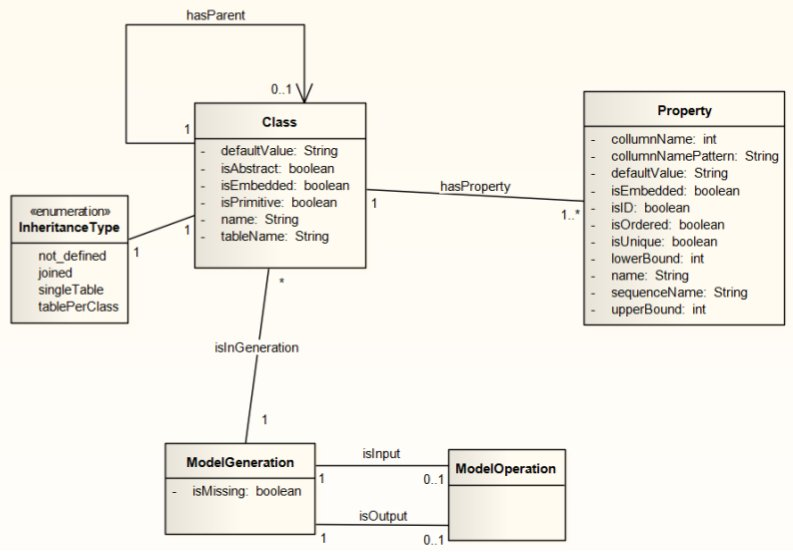
\includegraphics[width=15cm]{figures/app_meta_BP}
\caption{Aplikační metamodel v počátku vývoje obrázek převzat z \cite{Lukes}}
\label{fig:lukes:app_meta}
\end{center}
\end{figure}
%
\begin{figure}[h]
\begin{center}
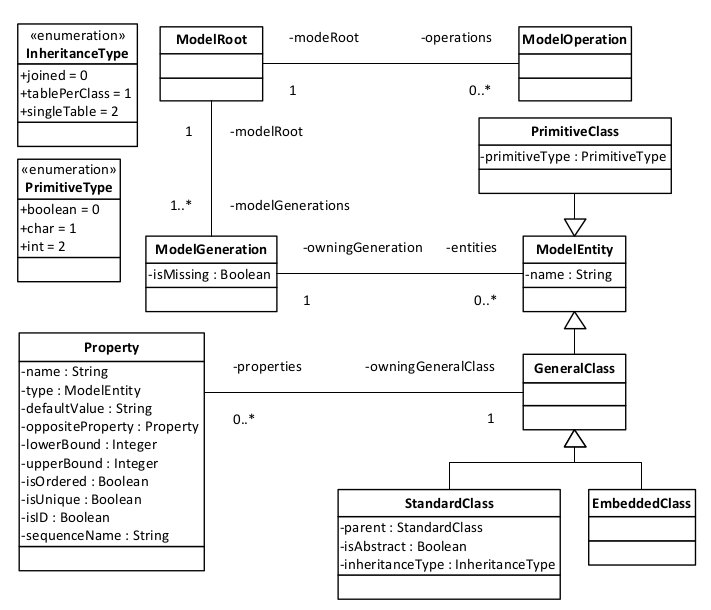
\includegraphics[width=15cm]{figures/app_meta_BP_jezek}
\caption{Aplikační metamodel v průběhu vývoje obrázek převzat z \cite{Jezek}}
\label{fig:jezek:app_meta}
\end{center}
\end{figure}
\FloatBarrier

\section{Změny aplikačních operací}
V průběhu modelování operací nad aplikačním modelem jsme se snažili, aby tyto
operace byly jednoznačné (strojově zpracovatelné) v rámci daného kontextu, dále
vzhledem k nutnosti textového zápisu uživatelem o minimalističnost zápisu. Tyto
dva koncepty jdou obecně proti sobě, proto jsme došli k jistému jejich
kompromisu uživatelské jednoduchosti zápisu a jednoznačnosti. Druhým cílem bylo
po odstranění kontrolního mechanismu a snaha o odstranění kontrolních queries,
které až při práci s instancemi dat zjistili, že daný skript vyvolá nad daty
chybu.

Operace v aplikačním modelu se vyvíjely a měnily se jejich parametry, ale
současně se měnil i seznam dostupných operací nad aplikačním modelem. Z operací
v první verzi modelu byly odstraněny operace MoveProperty, AddPrimitiveClass,
SetOpposite a SetType.

\subsection{Atomic, composed a virtuální operace}
V průběhu vývoje existoval entity ComposedOperation a AtomicOperation, kdy
každá operace byla buď composed nebo atomic, každá composed operace byla na
aplikační vrstvě nejdříve dekomponována na set atomických, které se později
vykonaly a mapovaly přes ORMo na databázové operace. Tento koncept jsme zavrhli,
protože jsme nedokázali dekomponovat správně některé operace a obzvláště
pořadí ORMo obrazů nám dělalo problémy. 

Některé nyní aplikované operace se rozkládají na operace virtuální na úrovni
kódu, nikoliv modelu, aby bylo zabráněno duplikaci kódu. Na první pohled se zdá
, že virtuální operace je obdobou Atomická operace, ale mezi těmito dvěma
koncepty existují dva rozdíly. Prvním rozdílem je, že pro atomické operace
vznikaly entity v modelu, což vedlo k jejich ukládání do mezivýsledných modelů a
bylo nutné je mazat. Druhým rozdílem je, že pro atomické operace se ověřovaly
validační podmínky, což se pro virtuální operace nedělá.

Koncept rozkladu operací na operace atomické se nedá považovat za špatný, ale je
nutné definovat širší množinu atomických operací - některé jen pomocné například
spojující třídy na základě nějakého kritéria. Tento čistší návrh podlehl nižšímu
množství práce na implementaci a měl za následek vyšší složitost testů.

\subsection{AddPrimitive} 
Operace AddPrimitive byla označena za nadbytečnou, protože není cílem modifikace
modelu změnit seznam primitivních tříd. Tento seznam bývá definován použitým
programovacím jazykem a tudíž by měl být ve vstupní generaci.

\subsection{SetOppositte}
V průběhu analýzy operace SetOpposite bylo zjištěno, že tato operace má smysl na
strukturální úrovni, ale stává se problematickou při práci s instancemi dat.
Operace bezproblémově funguje, pokud má odstranit nastavenou oppositeProperty,
tj. rozpojit oboustraně navigabilní vazbu. Pokud má operace naopak stvořit
oboustranně navigabilní vazbu, musí na aplikační úrovni zkontrolovat
existenci opozičních properties, zkontrolovat typy nastavovaných properties.
Strukturální kontrolu provede operace isValid(). Operace musí zkontrolovat, že
existují správné instance dat v databázi a spojit je. A v tom tkví problém této
operace. Bez znalosti instancí v databázi není možné najít takové mapování. Díky
odstranění kontrol při běhu skriptu nad databází není možné uživatele frameworku
upozornit na chybu v průběhu této operace.\\

Zdrojový stav máme zobrazený na obrázku
\ref{fig:finalization:setOpposite_source} a cílový stav Validační podmínky jsou
v pořádku.
Chceme dosáhnout stavu zobrazeného na obrázku
\ref{fig:finalization:setOpposite_target}. Řešením tohoto problému bylo
nahrazení operace SetOppositte dvojící operací ChangeBiToUnidir a
ChangeUniToBidir. Operace ChangeUniToBidir mění jednostranně navigabilní vazbu
přidáním property do třídy typu a nastavuje data opoziční property, operace tak
nepotřebuje kontrolovat, jaká data jsou v opoziční property, protože ta před započetím
operace neexistovala. Operace ChangeBiToUnidir pak odstraní oppositte atribut z
vlastnické property a odstraní samotnou property nesoucí data. Nechtěným, avšak
vítaným produktem této změny bylo zjednodušení vytváření oppositeProperty.
Původní plán počítal s operací AddProperty následovanou operací SetOppositte.
Nyní je možné dosáhnout tohoto cíle jedinou operací ChangeUniToBidir.
Zjednodušuje se i mazání oboustraně navigabilní vazby. V původní variantě bylo
nutné spustit operace SetOpposite s parametrem NULL pro opposite sloupec a
následně smazat opposite property operací RemoveProperty. Nyní tuto
funkcionalitu zajišťuje operace ChangeBiToUnidir.

\begin{figure}
\centering
\begin{subfigure}[b]{0.5\textwidth}
\fbox{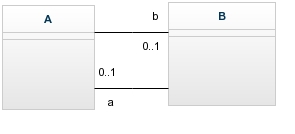
\includegraphics{figures/setOpposite_source}}
\caption{Stav před operací SetOpposite}
\label{fig:finalization:setOpposite_source}
\end{subfigure}
%
\begin{subfigure}[b]{0.5\textwidth}
\fbox{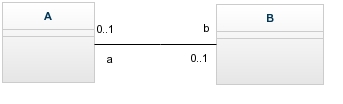
\includegraphics{figures/setOpposite_target}}
\caption{Výsledek po aplikaci operace SetOpposite}
\label{fig:finalization:setOpposite_target}
\end{subfigure}
\caption{Ilustrativní příklad k operaci SetOppositte}
\end{figure}
\FloatBarrier

\subsection{AddParent, RemoveParent}
V původním smyslu měla operace AddParent přidávat předka A třídě B, přičemž
třídy A a B neměly kolizní property. Z praktického pohledu je tato aplikace
operace AddParent nepoužitelná. Přidáváme-li existující třídu do hierarchie,
chceme získat vztah isA, který nám definuje, že třídy mají nejen společnou
funkcionalitu, ale téměř vždy i data. Představme si například, že modelujeme
grafický editor. V prvním kroku jsme vytvořili třídu Square, která má properties
area a side. Naprogramovali jsme kód používající třídu Square, vytvořili jich
několik, nakreslili\ldots a uložili. V druhé fázi jsme zjistili, že potřebujeme
více tvarů a tak jsme vytvořili třídu Circuit pro kruh. Následně jsme po napsání
kódu zjistili a uložení některých instancí Circuit do databáze, že
potřebujeme zacházet v některých případech pracovat s třídou Circuit stejně
jako s třídou Rectangle. Proto jsme extrahovali třídu Shape, předka třídy
Square. A v nynější chvíli nám operace ve frameworku Migdb nedostačují,
protože potřebujeme nastavit Shape jako rodičovskou třídu třídě Circuit, ale v
tom nám zabraňuje kolizní property. Na obrázku
\ref{fig:finalization:addParent_source} vidíme nynější stav. Tento stav jsme
vyřešili změnou validačních podmínek operace AddParent, kolizní property mohou
existovat. V zájmu jednoduchosti operace AddParent a jejího snadného zápisu v
jazyku Martina Mazance jsme nepřidávali kolizní property do signatury operace.
Operace je schopna si kolizní property dopočítat. 

Operace RemoveParent, inverzní operace AddParent, neví nic o původním stavu,
není schopna si původní kolizní property spočítat, takže její implementace se
změnila a tato operace kopíruje všechny property rodičovské třídy do potomka.
Slabinou v tomto přístupu je vznik nekonzistence inverze s původní operací viz
příklad nekonzistence uvedený v subsekci \ref{app_ops:removeParent_example}.

\begin{figure}
\centering
\fbox{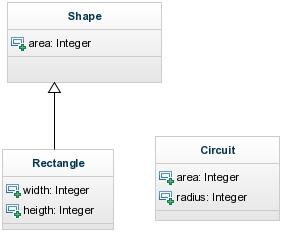
\includegraphics{figures/addParent_source}}
\caption{Model v průběhu vývoje aplikace}
\label{fig:finalization:addParent_source}
\end{figure}
\FloatBarrier


\subsection{SetType}
Operace SetType byla zkoumána, ale nebyla exaktně popsána, nebylo nalezeno
její mapování na operace v databázi ani validační podmínky nutné k úspěšné
aplikaci operace na aplikační model. Předpokládáme, že tato operace by měla být
aplikována na změny typu v hierarchii. Pokud by byla tato operace totiž
aplikována na primitivní typy, není možné kontrolovat data či dát uživateli
zprávu o nevalidnosti SQL skriptu.

\subsection{Vlastnosti operací}
V \cite{Cincetti} Antonio Cincetti popisuje některé specifické vlastnosti
jako je invertovatelnost a rozložitelnost operací. Je nutné říci, že operace
zmiňované v literatuře pracují jen se strukturou dat, nikoliv s daty samotnými
a jsou kontextově nezávislé - tyto operace jsou tvořeny téměř výlučně
konstruktivními a  destruktivními operacemi. Cincetti rozděluje zmiňuje, že v
minulosti byly operace aplikovatelné na jeden konkrétní model (intensional) a
modernější differenční modely jsou tzv. extensional - je možné je aplikovat na
jakýkoliv model, například na paralelní vývojové větve.

V projektu Migdb jsou operace invertovatelné se znalostí původního modelu.
Například u operace RemoveParent(childClass) nezískáme parentClass přímo z
operace, ale musíme ho dopočítat ze vstupního modelu.

\label{app_ops:removeParent_example} Problémem je, že i po odvození inverze
nemusí vést aplikace operace do stejného vstupního modelu. Pokud například na
stav \ref{fig:add_parent} aplikujeme operaci AddParent(Teacher,
UniversityTeacher), získáme cílový stav
\ref{fig:remove_parent}. Pokud se chceme vrátit zpět z \ref{fig:remove_parent}
do výchozího stavu, měli bychom aplikovat operaci
RemoveParent(UniversityTeacher), nicméně aplikace této operace nepovede do
výchozího stavu \ref{fig:add_parent}, ale do stavu \ref{fig:remove_parent_apl}.
Po aplikaci operace RemoveParent bude v třídě UniversityTeacher navíc property
class. Tento stav je zapříčiněn vývojem operace AddParent - v původní verzi
operace nemohla být použita na jakékoliv třídy s kolizními atributy, ale
shledali jsme tuto operaci nepoužitelnou - většinou přidáváme supertyp třídě,
pokud je třída potomka speciálním typem třídy rodičovské, což se ale v
drtivé většině případů projevuje kolizními atributy. Možným odstraněním tohoto
problému by bylo přidání informací o distribuovaných properties do operace
RemoveParent, čímž bychom se nicméně odklonili od cílu minimalizovat operace.

\begin{figure}
\centering
\begin{subfigure}[b]{0.33\textwidth}
\fbox{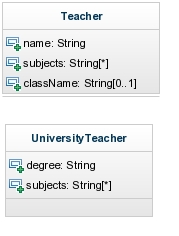
\includegraphics{figures/teacher_university_teacher_a}}
\caption{AddParent(Teacher, UniversityTeacher)}
\label{fig:add_parent}
\end{subfigure}
%
\begin{subfigure}[b]{0.33\textwidth}
\fbox{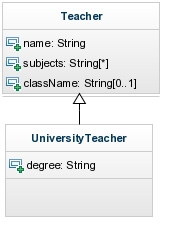
\includegraphics{figures/teacher_university_teacher_b}}
\caption{Výsledek po aplikaci operace AddParent}
\label{fig:remove_parent}
\end{subfigure}
%
\begin{subfigure}[b]{0.33\textwidth}
\fbox{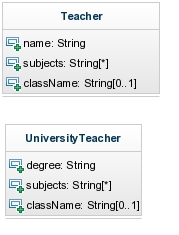
\includegraphics{figures/teacher_university_teacher_c}}
\caption{Výsledný stav po aplikaci RemoveParent}
\label{fig:remove_parent_apl}
\end{subfigure}
%
\caption{Ukázka operace AddParent}
\end{figure}

\FloatBarrier

\section{Změny Databázového Struktury}
 Metamodel databázové struktury se ukázal jako celkem dobře definovaný a proto
 nedocházelo k zásadním změnám.

 Na obr. \ref{fig:rdb_str} vidíme aktuální matamodel databázové struktury, na
 obr. \ref{fig:rdb_str_lukes} vidíme model na počátku vývoje převzatý z
 \cite{Lukes} a na obrázku \ref{fig:rdb_str_tarant} model v pozdější fázi vývoje
 převzatý z \cite{Tarant_bp}.

 Nejvýraznější změnami databázového metamodelu struktury jsou - stejně jako v
 metamodelu aplikační struktury odstranění generace modelů, odstranění elementu
 UnderlyingIndex, odstranění elementu ColumnConstraint, nahrazení elementu
 NotNullConstraint atributem boolean v Column a snížení kardinality Sequence
 obsažených ve schematu z * na 1.
 
 Myšlenka generace modelů byla zachována, ale jejich připadné uchovávání bylo
 zvoleno ve více oddělených souborech. Element UnderlyingIndex byl shládán
 nadbytečným, stejně jako element ColumnConstraint. Neatributový element
 NotNullConstraint byl shledán příliš informačně chudým a byl nahrazen atributem
 isNillable zachovávajícím stejnou informační hodnotu jako element v původních
 modelech. 

\begin{figure}[H]
\begin{center}
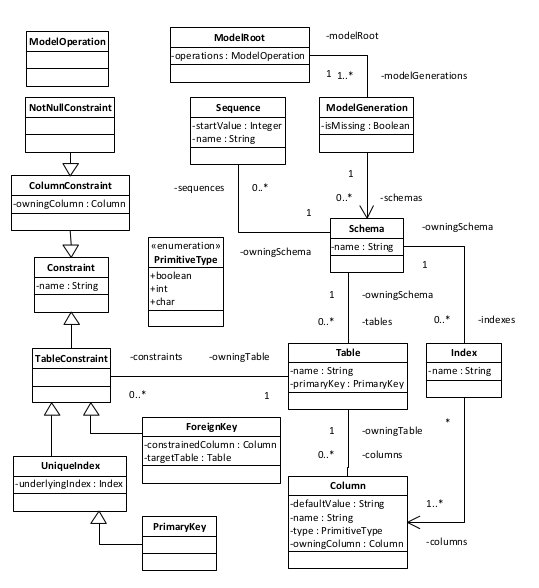
\includegraphics[width=10cm]{figures/rdb_structure_tarant}
\caption{Struktura databázového metamodelu v průběhu vývoje, obrázek převzat z
\cite{Tarant_bp}}
\label{fig:rdb_str_tarant}
\end{center}
\end{figure}
%
\begin{figure}[H]
\begin{center}
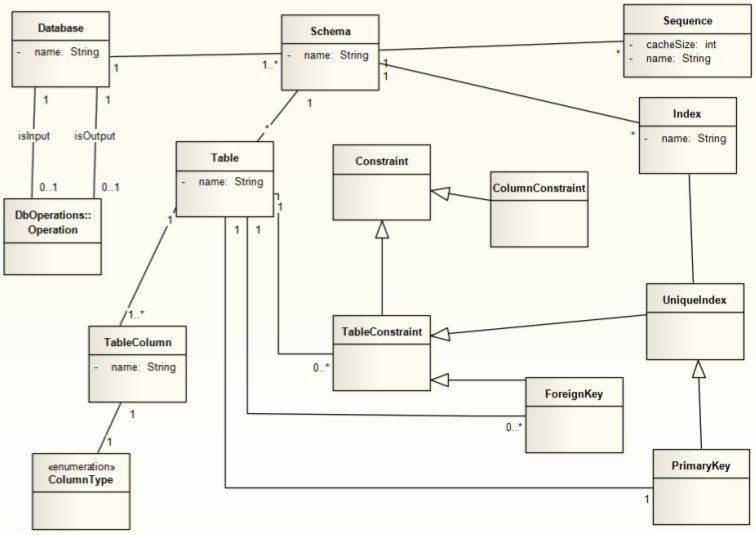
\includegraphics[width=15cm]{figures/rdb_structure_lukes}
\caption{Struktura databázového metamodelu v průběhu vývoje, obrázek převzat z
\cite{Lukes}}
\label{fig:rdb_str_lukes}
\end{center}
\end{figure}
%
\FloatBarrier

\section{Změny databázových operací}

Databázové operace v původní verzi byly designově nečisté, některé operace
obsahovaly ve své definici odkazy na entity z modelu aplikačního, které již v
modelu databázovém neexistují a ani nemohou existovat. Mou prací na databázových
operacích bylo odstranění entit aplikace, které v databázovém metamodelu již
nemohou existovat a dodefinovat potřebné obecně použitelné operace.

\subsection{AddSchema a RemoveSchema}
Operace AddSchema a RemoveSchema byly odstraněny. Pro každou tabulku je
definováno, ve kterém schematu se nalézá, ale neexistuje aplikační operace,
která by zapříčinila vznik nebo smazání databázového schematu.

\subsection{HasNoInstances, HasNoOwnInstances}
Operace HasNoInstances měla zjistit, jestli v dané tabulce existují data.
Operace HasNoOwnInstances zjišťovala, jestli v tabulce odpovídající třídě A
existují data odpovídající konkrétní instanci A, nikoliv data odpovídající
instancím jejích potomků.
Tyto dvě operace byly napsány jako základ ověřování proveditelnost migrovaných
skriptů, který byl z frameworku vypuštěn. Pokud by se měl do frameworku
navrátit, bylo by lepší namodelovat jednu operaci HasNoInstances s where
podmínkou vybírající daná data.

\subsection{GenerateSequenceNumbers}
Operace GenerateSequenceNumbers byla shledána nadbytečnou, protože při vkládání
dat je možné generovat je ze sekvence přidružené k tabulce či specifikované v
parametru. Není tedy nutné vkládání dat do tabulky oddělovat od Generování data
ze sekvence.

\subsection{AddIndex, RemoveIndex}
Z databázového metamodelu byl odstaněn element Index. Některé operace sice
vytvářejí defaultní index, ale k tomuto vytvoření stačí jejich samotné zavolání.
Z těchto důvodů byly operace z metamodelu odstraněny.

\subsection{SetColumnType}
Operace SetColumnType měla konvertovat data z jednoho primitivního typu na
druhý. V nynější chvíli není aplikační operace, která by se na tuto databázovou
operaci mapovala a je očekávané, že aplikační operace SetType bude měnit
neprimitivní typ. Operace se tedy stala nadbytečnou a byla z modelu odstraněna.


\subsection{UpdateRows}
V původní verzi měla tato operace signaturu:

\begin{verbatim}
    class UpdateRows extends ModelOperation {
      attr String[1] owningSchemaName;
      attr String[1] sourceTableName;
      attr String[1] sourceColumnName;
      attr String[1] targetTableName;
      attr String[1] targetColumnName;
      attr ToleranceType[1] tolerance;
      attr String[1] idName;
    }
\end{verbatim}

Na verzi nynější:

\begin{verbatim}     
     class UpdateRows extends ModelOperation {
      attr String[1] owningSchemaName;
      attr String[1] sourceTableName;
      attr String[1] sourceColumnName;
      attr String[1] targetTableName;
      attr String[1] targetColumnName;
      attr String[1] selectionWhereCondition;
      attr String[?] safeWhereCondition;
    }
    \end{verbatim}
Shledal jsem nadbytečným atribut ToleranceType, jelikož jeho přesný význam nebyl
definován a nebyl použit v ORMo mapování. V operaci byl nahrazen atribut idName
atributem selectionWhereCondition. Testy odhalily, že je nutné přidat volitelný
atribut safeWhereCondition, aby byla zajištěna neměnnost instancí dat, které
operace nemá změnit.

\subsection{DeleteRows}
Signatura operace byla změněna z verze:
\begin{verbatim}
    class DeleteRows extends ModelOperation {
      attr String[1] owningSchemaName;
      attr String[1] tableName;
      attr String[*] descendantsNames;
      attr String[1] idName;
    }
\end{verbatim}
Na verzi:
\begin{verbatim}
   class DeleteRows extends ModelOperation {
      attr String[1] owningSchemaName;
      attr String[1] tableName;
      attr String[1] whereCondition;
    }
\end{verbatim}  
Výstupní verze je čitelnější, obecněji použitelná a designově čistší.

\subsection{NillRows}
Motivací k vytvoření této operace bylo shledání potřebného nastavování
NULL hodnoty v cílové tabulce. Operace nebyla shledána jako speciální typ
UpdateRows, jelikož operace neaktualizuje data v cílové tabulce na základě
zdrojové tabulky.

\subsection{InsertRows}
Do operace byl přidán atribut whereCondition, aby byla operace lépe použitelná.

\subsection{RemoveNotNull}
NotNull constraint byl zpočátku vývoje chybně zařazen mezi TableConstraints a
bylo předpokládáno, že je odstranitelný operací RemoveConstraint. Po zjištění
neplatnosti tohoto předpokladu jsem vytvořil tuto operaci.

\section{Databázová evoluce, Aplikační Evoluce a Migdb\_Executor}
Evoluce na databázové vrstvě nemá vliv na vygenerování SQL kódu a je jen
jakousi simulací změn, které se provedou na databázové vrstvě, tudíž se může
jevit nadbytečnou. Nicméně tato simulace může odhalit chyby ve vygenerovaném
SQL skriptu podstatně rychleji oproti generování databáze a aplikaci migračních
skriptů, které jak z praxe víme často probíhají v řádu desítek minut až
několika hodin. Proto jsem se rozhodl tuto část zachovat ve frameworku.

\subsection{Sekvenční představa}
Původní představa o funkci frameworku Migdb je zobrazena na obrázku
\ref{fig:framework_seq}. Problémem tohoto návrhu je úplná sekvenčnost zpracování
jednotlivých kroků. V prvním kroku se všechny aplikační operace aplikují na
vstupní model. V druhém kroku se tyto operace transformují pomocí ORMo modulu na
databázové operace. Díky závislosti ORMo mapování na aktuálním aplikačním
modelu zde může nastat problém. Pokud budeme mít sekvenci operací $O_1,\ldots
O_n$, která pozmění aplikační model na model $M_1$ tak, že některá z operací
nebude validní, transformace ORMo nemusí dávat korektní výstup. Příklad této
anomálie je aplikace operací SetBounds(1, 1), RemoveProperty(\uv{C}, \uv{P}).
Pokud aplikujeme na model obsahující třídu \uv{C} s Property \uv{P} tyto dvě
operace, pak v cílovém modelu nebude existovat Property \uv{P}, kterou
transformace ORMo potřebuje k namapování operace SetBounds.

\begin{figure}[H]
\begin{center}
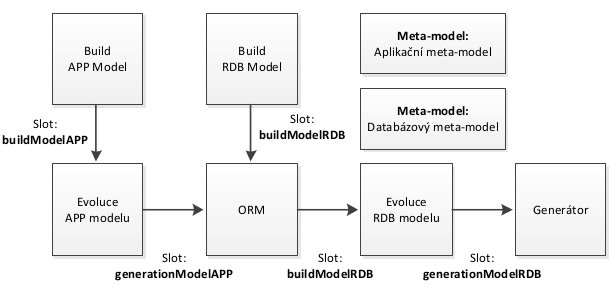
\includegraphics[width=13cm]{figures/framework_cycle}
\caption{Původní sekvenční představa. Převzato z \cite{Tarant_bp}}
\label{fig:framework_seq}
\end{center}
\end{figure}

\FloatBarrier

\subsection{Změny SQL generátorů}
Vzhledem k změnám databázových operací bylo nutné upravit i generátor SQL kódu z
těchto operací. Druhou podstatnou prací bylo přepsání základního algoritmu pro
vytvoření databázového schematu z aplikačního modelu použitého v mé bakalářské
práci viz \cite{Lukes}, aby bylo možné napsat testy celého frameworku. Byly
naimplementovány metody apply pro operace:




\section{Implementace a testování ORMo mapování}
Nejnáročnější implementační částí bylo napsání ORMo mapování a jeho testů.
Původní implementace prezentovaná v Cambridge se ukázala jako velmi neflexibilní
, špatně rozšířitelná a testovatelná. Proto jsem téměř celou ORMo implementaci
přepsal. Implementace ORMo zabírá přes 2000 řádků kódu. Vzniklo 42 testů ORMo
mapování.

\subsection{Mapování jmen}\label{subsect:map_translation}
ORMo mapování udržuje konzistenci mezi aplikačním modelem a modelem databázovým.
Databáze umožňuje definovat nepojmenované constrainy, ale aby bylo možné smazat
TableConstrain je nutné ho referencovat pomocí jeho jména. Databáze
neumožňují měnit název TableConstrainů a tak je každou změnu názvu jména
TableConstrainu nutné reprezentovat jako odstranění a jeho opětovné vytvoření.
Aby ORMo mapování zajistilo konzistenci mezi aplikačním a databázovým modelem,
bylo nutné zajistit jednoznačné mapování mezi elementy aplikační vrstvy a
elementy databázovými. Kritickým problémem se stalo mapování jmen. Vznikla
knihovna name\_service, která tento problém řeší. Jména tříd je jednoduché
transformovat na jména tabulek pomocí následujících pravidel:

\begin{itemize}
  \item Počáteční písmeno je zmenšeno
  \item Každé další velké písmeno je nahrazeno malým písmenem stejného typu
  předraženého znakem "\_"
\end{itemize}

Stejná pravidla jsou použita při transformaci primitivních properties s
upperBound 1 na sloupce. Tedy třída LegalPerson(businessName,
registrationNumber) se transformuje na tabulku legal\_person(business\_name,
registration\_number). Použití daných dvou pravidel označme jako volání funkce
translate na daný název.

Při transformaci asociačních property s upperBound != 1 na asociační tabulku je
nutné zajistit unikátnost názvu této tabulky. Neexistuje předpoklad, že by byl
název property unikátní ve všech třídách. Ale dvojice (table, property) musí být
unikátní. Proto je název asociační tabulky získán jako spojení názvu vlastnické
tabulky s názvem asociační property pomocí znaku "\_". 
$$owningTableName = translate(owningClassName)$$
$assocTableName = owningTableName$ + "\_" +
$translate(associationPropertyName)$

Transformace primitivní property s upperBound != 1 (kolekce) na tabulku má
podobný důsledek. Aby bylo pro vývojáře snadnější rozpoznat obraz třídy kolekce
je název tabulky předražen prefixem "col\_"

$$owningClstranslation = translate(owningClassName)$$
$$propertyTranslation = translate(primitivePropertyName)$$
$collectionTableName = $"col\_" $+ owningClsTranslation + $"\_" $+
propertyTranslation$

Názvy constrainů musí být unikátní v rámci celé databáze. Toto je
zajištěno. Názvy unique constrainů jsou odvozeny od tabulky, nad kterou je
constrain vytvořen. Existují dva atributy, které jsou mapovány na 
UniqueConstraint. Aplikační atribut kolekce isUnique je mapován na
UniqueConstraint s jménem předraženým "ux\_". Název constraintu pro
atribut isOrdered je předražen řetězcem "ux\_" a nakonec je doplněn
řetězec "\_ord".
Vzhledem k unikátnosti dvojice (class, property) bylo využito mapování prefix
spojený s přelozeným názvem třídy a přeloženým názvem property.
$$owningClstranslation = translate(owningClassName)$$
$$propertyTranslation = translate(primitivePropertyName)$$
$uxName = $"ux\_" $+ owningClsTranslation + $"\_" $+
propertyTranslation$
$ordName = uxName + $"\_ord"

Relace parent je do databáze transformována jako cizí klíč. Vzhledem k
zákazu vícenásobné dědičnosti je každá relace parency nad tabulkou
jednoznačně určena vzorem této tabulky. Tento klíč má proto jméno odvozeno od
přeloženého názvu třídy předražené řetězcem "par\_".

$ parentFkName = $"par\_" $+ translate(owningClassName)$

Tabulka kolekce referencuje vlastnickou tabulku právě jednou a název cizího
klíče je tedy odvozen z názvu tabulky kolekce.

$fkCollectionName = $"fk\_" $+ collectionTableName$

Poslední pravidlo vytváření cizích klíčů platí pro asociační tabulky. Každá
asociační tabulka referencuje právě dvě tabulky. Název cizího klíče je vytvořen
z názvu asociační tabulky a tabulky, kterou referencuje předražený řetězcem
"fk\_".

$fkAssociationReference =$"fk\_" $+ associationTableName + $"\_"$ +
referencedTableName$


Tato pravidla nezajišťují unikátnost jmen elementů ve všech případech, ale
zajišťují unikátnost jmen ve všech skupinách. Celkovou unikátnost jmen zajistí
dobrý návrh aplikace a zkontroluje Databázová evoluce.

\chapter{Řešení problému rozpoznávání operací}\label{chapt:recognition}

Dalším cílem, který jsem si před vypracováním diplomové práce stanovil bylo
vytvoření a zdokumentování algoritmu generující z dvou vstupních modelů
sekvenci operací, jejichž aplikací se model zdrojový transformuje na model
koncový.

\section{Diff a delta notace}
Nejznámějším nástrojen používaným při porovnávání a zjišťování změn dvou
textových souborů tzv. patchů \cite{patch} je nástroj diff \cite{diff_wiki} .
Diff je založen na algoritmu hledání největší společné podsekvence (LCS) viz
\cite{wiki_lcs}. Algoritmus LCS byl analyzován a nebyl shledán jako dostatečným
pro námi definovaný problém, jelikož nezohledňuje doménu problému. Výstup
algoritmu se dá vyjádřit pomocí delta notace.

Příklad Delta notace za pomoci linuxových
nástrojů diff dvou souborů najdeme na výpisu \ref{Patch_1_2} \\
\begin{lstlisting}[language=JAVA,frame=single,caption=Man1.java,label=Man1]
class Man {
	private String name;

	public Man(String name){
		this.name = name;
	}

}
\end{lstlisting}

\begin{lstlisting}[language=JAVA,frame=single,caption=Man2.java,label=Man2]
class Man {
	private String name;

	private String surname;

	public Man(String name){
		this.name = name;
	}

	public Man(String name, String surname){
		this(name);
		this.surname = surname;
	}
}
\end{lstlisting}

\begin{lstlisting}[language=JAVA,frame=single,caption=Patch Man1
Man2,label=Patch_1_2]
3a4,5
> 	private String surname;
> 
5a8,12
> 	}
> 
> 	public Man(String name, String surname){
> 		this(name);
> 		this.surname = surname;	
\end{lstlisting}

Ukázka kódu \ref{Man1} zobrazuje zdrojový kód třídy Man v první
verzi. Ukázka \ref{Man2} potom zdrojový kód třídy Man po první naší editaci,
kdy jsme do dané třídy přidali nový atribut a nový konstruktor.
Diff v delta notaci těchto dvou souborů je ukázán v \ref{Patch_1_2}. V delta
notaci vidíme, že do prvního souboru byly za 3. řádek vloženy řádky 4-5 z
druhého souboru - řádek definující nový atribut surename a oddělující prázdný
řádek, dále za 5. řádek byly vloženy řádky 8-12 z druhého souboru definující
nový konstruktor a uzavírací závorka.\\

V \cite{Cincetti} jsou definovány operace pomocí delta notace. Delta notace
ukazuje všechny změny mezi danými dvěma artefakty stejné úrovně abstrakce.
Změnami můžeme rozumět přidáním elementu, odstraněním elementu a modifikací elementu.

Delta notace je dle autora výhodná díky snadné rozložitelnosti velkých patchů na
více menších patchů. Druhá výhoda je použitelná při paralelním vývoji. Pokud
vznikne více verzí souboru v různých větvích, delta notace umožňuje snadné
oddělení konfliktních operací od operací nezávislých.

Delta notace vytvořená dle metamodelu na obr. \ref{fig:diff_cincetti} definuje
add, delete entit a modify atributů jednotlivých entit. V našem modelu existují
operace, které se nedají zařadit ani do skupiny add, delete a modify operací.
Operace ExtractClass, ExtractSuperClass, InlineClass, CollapseHierarchy,
PullUpProperties a PushDownProperties naopak nepatří mezi modifikační, add ani
delete operace.
proto jsme mohli postupovat jednou z následujících cest

\begin{itemize}
  	\item získat standardní diff dvou modelů a aplikovat na něj algoritmus
  	rozpoznávání jakožto sadu podmínek, které musí platit, aby algoritmus rozpoznal operaci.
	\item vytvořit vlastní Diff metamodel, který podobně jako v
	\ref{fig:diff_cincetti} odpovídá vlastnímu seznamu operací aplikovatelých na
	model.
\end{itemize}

Zvolili jsme si cestu definice vlastního metamodelu.

\begin{figure}[H]
\begin{center}
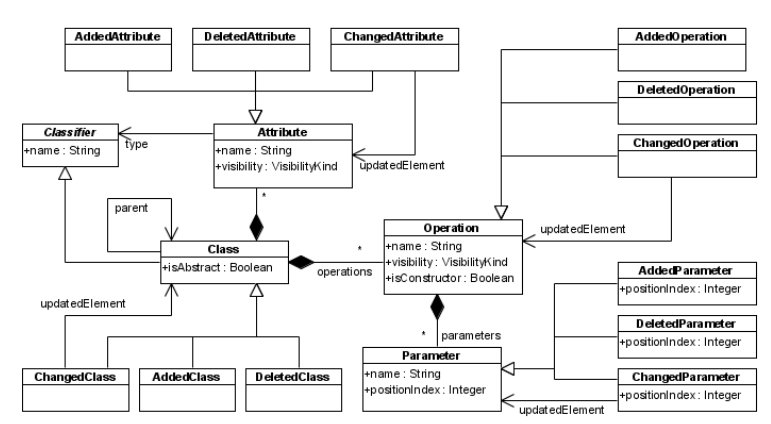
\includegraphics[width=15cm]{figures/uml_diference_cincetti}
\caption{Diff model převzatý dle \cite{Cincetti}}
\label{fig:diff_cincetti}
\end{center}
\end{figure}

\begin{figure}[H]
\begin{center}
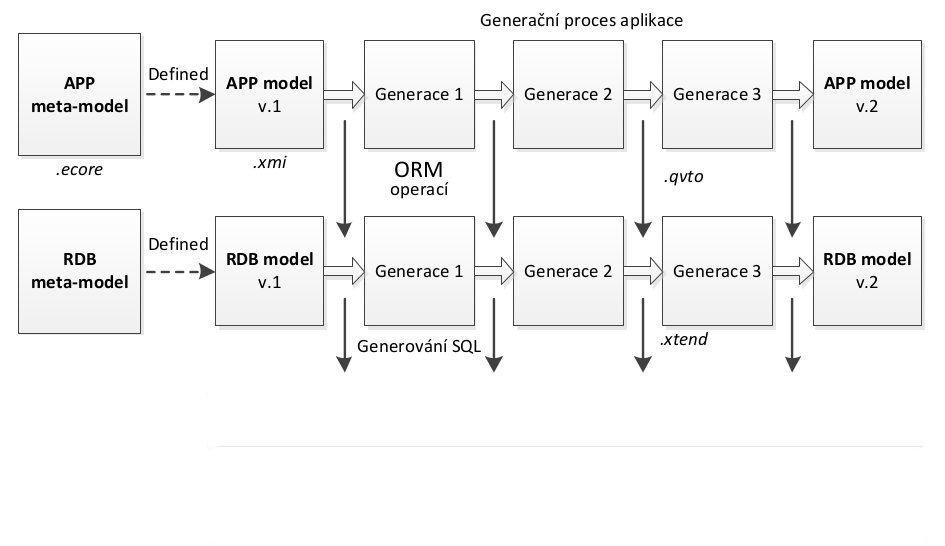
\includegraphics[width=15cm]{figures/framework_structura_tarant_modified}
\caption{Seznam diff elementů}
\label{fig:diff_meta}
\end{center}
\end{figure}

\FloatBarrier

\section{Rozpoznávání operací}

Algoritmem pro rozpoznávání operací nazveme každý algoritmus, který nám pro
každý vstupní model A a cílový model B najde uspořádaný seznam operací, jejichž
postupná aplikace transformuje model A do modelu B. Tento algoritmus nemusí být
deterministický.

Jedním z zajímavých faktů je poznatek, že seznam operací nemusí být jednoznačný
a to i u jednoduchých změn. Pokud aplikujeme sekvenci operaci Inline A, B + 
Rename B ->C na model X dostaneme stejný výstup jako aplikací operací Inline B,
A + Rename A->C, ještě zajímavějším poznatkem je, že nejsme schopni rozeznat
rozdíl mezi aplikací sekvence operací Rename A, C + Inline C, B.

Samostatným tématem je pořadí operací a jeho permutace. Je zřejmé, že pořadí
transformací v seznamu operací operujících nad hierarchiemi dědičnosti bude
možné libovolně prohazovat.
Také je samozřejmé, že seznam reduktivních operací stejného typu je také možné
libovolně zpermutovat. Stejně tak seznam aditivních operací stejného typu.
Obecný princip permutability kolekce operací není znám. 

\section{Obecné principy model matching} \label{model_matching_principles}
Nejtriviálnější implementovatelný algoritmus by mohl smazat zdrojový model
pomocí destruktivních operací a následně vytvořit výsledný model pomocí operací
konstruktivních, připadně poupravit atributy jednotlivých elementů pomocí
operací modifikačních. Argumentem proti použití takového algoritmu je smazání
jakýchkoliv dat, které v původní databázi byla. Takovýto algoritmus tudíže
nemigruje žádná data, ale nahrazuje funkci ORM mapování integrované
do většiny současných IDE. Proto se jím v této práci nezaobírám.

Jak je diskutováno v \cite{diff_merge_diagrams} a
\cite{Kolovos:Different_models} existuje několik požadavků na algoritmus řešící
problém model matching. Tyto požadavky zahrnují přesnost, vysokou míru
abstrakce na které je porovnávání provedeno, nezávislost na konkrétních
nástrojích, doménách a jazycích, použitelnost a minimální nutnost adaptace
algoritmus pro daný problém. Tyto požadavky jdou proti sobě a je nutné
preferovat některé na úkor jiných, proto není možné označit za nejlepší, ale je
nutné vybrat si správný algoritmus v závislosti na řešeném problému.

 V \cite{Kolovos:Different_models} byly popsány algoritmy
 pro mapování shodných entit modelů a algoritmy pro získávání rozdílu modelů. 
 Principem těchto modelů je párování elementů vstupního modelu s elementy z
 modelu cílového. Autor je dělí na 4 obecné skupiny matching algoritmů.
 
 \begin{itemize}
   \item Párování podle statického identifikátoru páruje elementy podle
 	perzistentního identifikátoru, který je přiřazen každé entitě v době jejího
 	vzniku, je neměnný a unikátní. Nejzákladnějším principem model matchingu je
 	tedy párování entit na základě shodnosti jejich identifikátorů. Tento princip
 	má výhody jednoduchosti implementace a rychlosti. Tento algoritmus není
 	použitelný pro modely vytvořené nezávisle jeden na druhém či u technologií
 	nepodporujících údržba unikátních identifikátorů.
 
 	\item Algoritmus signature based matching byl navržen kvůli limitaci párování
 	podle statického identifikátoru, tento algoritmus je založen na dynamickém
 	vypočtení nestatické signatury jednotlivých elementů pomocí uživatelem
 	definovaných funkcí specifikovaných pomocí nějakého dotazovacího jazyka.
 	Tento princip tedy může být použit pro modely vzniklé nezávisle na sobě.
 	Nevýhodou je potom nutnost specifikovat query, které dopočítají signaturu.
 
 	\item Algoritmus Similarity based matching používá podobně jako signature
 	based matching podobnost sublementů jednotlivých elementů, kterou agreguje do
 	skalární hodnoty. Tento princip se řadí mezi podtyp attribute graph
 	\cite{attributed_graph} matchingu.
 	Každá feature modelu může mít jinou váhu pro porovnávání, napřiklad u
 	podobnosti tříd má jméno vyšší důležitost nežli abstraktnost dané třídy. 
 	Tento algoritmus musí být typicky doplněn o konfiguraci vah jednotlivých
 	features elementů, kterou většinou píše vývojář. Zástupcem tohoto principu je
 	framework EMF Compare, který je doplněn o defaultní konfiguraci vah. Výhodami
 	je větší přesnost, nevýhodou je potom TRIAL ERROR (pokus omyl) metoda
 	získávání vhodné konfigurace vah.
 
	\item \label{UML_Diff} Algoritmy v kategorii Custom language specific matching
	jsou vytvořené přímo k využití daného modelovacího jazyka. Hlavní výhodou je, že
 	algoritmus na dané doméně může začlenit do metody similarity based matchingu
 	sémantické detaily, což vede k přesnějším výsledkům a redukuje prohledávaný 
	stavový prostor. Jako příklad je uváděn jazyk UMLDiff, který při porovnávání
	dvou UML modelů může využít faktu, že dvě třídy nebo dva datové typy
	stejného jména tvoří po všech praktických stránkách pár(match). Nicméně výhoda
	začlenění sémantických detailů konkrétní domény je vykoupeno vysokou cenou -
	všechny ostatní kategorie algoritmů potřebují minimální neb téměř žádné úpravy
	od vývojáře, pro tuto kategorii vývojáře musí napsat celý matchovací algoritmus
	sám.
\end{itemize}

\section{Graph matching}
 Problém model matching je podproblémem generičtějšího problému graph matching, 
 který studuje \cite{bengoetxeaPHD02} a rozděluje a popisuje algoritmy pro
 graph matching - algoritmus nalezení shody grafů. Problém je definován na
 obecné struktuře Graf, což je uspořádaná dvojice G = (V, E), kde G je množina
 uzlů a E je množina hran grafu, přičemž $E \subset V \times V$. Grafy mohou
 být orientované či neorientované, mohou mít vícenásobné hrany.
 
 Každý graf může přidávat informace do své struktury pomocí labelu (popisku
 nebo čísla) do hran a vrcholů, pokud je nutné přidat více informací, je možné
 přidat do hran a/nebo vrcholů atributy, potom hovoříme o vertex-atributed
 grafech a edge atributed grafech, případně attributed grafech. V některé
 literatuře jsou attributed grafy označovány jako labeled grafy. Graph
 matching je aplikován v mnoho oborech jako je počítačové vidění, analýza
 scény (scene analysis), chemie a molekulární biologie. Pro tyto obory je
 esenciálním nalézt vzorky nalezeny v daných datech. 
  
 Problém shodnosti dvou grafů $G_O$ (grafu originálu) a $G_V$ (grafu
 vzorku), se dělí na algoritmus nalezení přesné shody vzorku v hledaném grafu
 či algoritmus hledání podobnosti grafu vzorku v hledaném grafu jak je zobrazeno
 na obr. \ref{fig:graph_matching} převzatém z \cite{bengoetxeaPHD02}.
 
 Algoritmus hledání přesné shody je definován následně: Mějme grafy $G_O = (V_O
 , E_O)$ a $G_V = (V_V, E_V)$, přičemž $\| V_O\| = \| V_V\|$, úkolem je potom
 najít takové prosté zobrazení  $f: V_O \rightarrow V_V$, takové, že $(u, v) \in
 E_O$ iff $(f(u), f(v)) \in E_V$. Pokud takové mapování existuje, nazveme ho
 přesnou shodou. \\
 
 Termín Hledání podobnosti grafů (inexact macthing) aplikovaný na některé
 problémy týkající se shodnosti grafů vyjadřuje, že není možné nalézt
 izomorfismus mezi dvěma grafy, aby byly shodné. V těchto případech mají grafy
 rozdílné charakteristiky jako je například jiný počet vrcholů, jiný počet hran
 či jiná délka nejdelší kružnice.
 Tedy není hledán izomorfismus dvou grafů, ale problém je upraven na hledání
 největší možné shody mezi grafy.
 Tato transformace mění problém a zařazuje ho do třídy problémů známé jako
 inexact graph matching.
 V takovém případě hledáme nebijektivní korespondenci mezi grafem vzorku a grafem
 originálu. V následujícím textu předpokládejme $\|V_V\| < \|V_O\|$. Inexact
 matching je používán v oborech kartografie, rozpoznávání znaků a medicíně.
 Nejlepší korespondence graph matching problému je definována jako optimum
 nějaké objektivní funkce, ktérá měří podobnost mezi přiřazenými uzly a
 hranami. Tato funkce je nazvána fitness funkcí, případně funkcí energie.

 Formálně je tedy hledání podobnosti grafů definováno takto: mějme dva grafy,
 $G_V a G_O$ přičemž $\| V_V \| < \| V_O\|$ a cílem je nalezení mapování $f' :
 V_D \rightarrow V_M že (u, v) \in E_P$ iff $(f(u), f(v)) \in E_M$.\\
 
 Podtypem těchto úloh jsou problémy subgraph matching a subgraph izomorfizmu.
 
 Při hledání složitost uváděných problémů autor \cite{bengoetxeaPHD02} řadí
 hledání přesné shody do P až NP kompletní množiny úloh, přičemž že u problémů
 této kategorie nebyla dokázána nejvyšší složitost NP complete. Pro problémy
 subgraph isomorphismu bylo dokázáno, že patří do třídy NP complete. Pro
 složitost nepřesného graph matchingu bylo dokázáno, že patří do třídy NP-complete.
  
 \begin{figure}[H]
\begin{center}
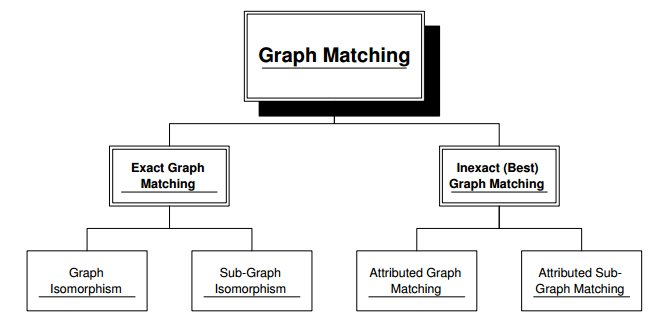
\includegraphics[width=15cm]{figures/graph_matching.jpg}
\caption{Typy graph matchingu}
\label{fig:graph_matching}
\end{center}
\end{figure}
 
\FloatBarrier
 
 \chapter{Vytvořené algoritmy rozpoznávání
 operací}\label{chapt:recognition_implementation}

\section{Stavový algoritmus}\label{sec:algo_state}

V ranné fázi jsem napsal prototyp rozpoznávacího algoritmu, který se snaží 
minimalizovat vzdálenost současného modelu od modelu cílového pomocí rozpoznání
operací a jejich následné aplikace. Výhodou tohoto přístupu je možnost nalezení
více alternativních cest, nevýhodou je potom velikost stavového prostoru
zvětšující se s počtem rozpoznávaných operací. Algoritmus je popsaný v
pseudokódu viz algoritmus \ref{algo:state}
%\\

Algoritmus v prvním svém kroku inicialializuje hodnoty.
Aktuálnímu modelu nastaví hodnotu modelu zdrojového. Množinu rozpoznaných
operací $R_{ops}$ inicializuje prázdnou množinou. Rozpoznanou R operaci nastaví
na NULL.

Následně opakuje cyklus repeat začínající na řádce \ref{algo:state:repeat},
který je ukončen splněním terminální podmínky uvedené v pseudokódu na řádce
\ref{algo:state:terminal_condition}, R = NULL. Tj. algoritmus je ukončen, pokud
v těle cyklu nebyla rozpoznána žádná operace.

V těle cyklu Repeat potom algoritmus nastaví hodnotu R na NULL a nastaví
na zmíněném řádku \ref{algo:state:improvement} hodnotu aktuálního nejlepšího
zlepšujícího kroku K na 0, aby zajistil přemazání dat nalezené operace v minulé
iteraci cyklu.

Algoritmus spočítá v cyklu na řádcích
\ref{algo:state:forOps}-\ref{algo:state:forOpsEnd} pro každou operaci maximální
zlepšující krok této operace $K_{op}$. Pokud je $K_{op}$ lepší než
dosavadní maximum K, aktualizuje $K_{op}$ a R. Následně algoritmus v případě
rozpoznání nějaké operace - viz. řádek \ref{algo:state:addOp} nalezne parametry
params pro operaci R viz metoda getParams(R, A, S) na řádku
\ref{algo:state:getParams}. Tato metoda by například pro operaci AddClass
nalezla jméno třídy, která neexistuje v zdrojovém modelu, ale existuje v cílovém
modelu. Algoritmus přidá operaci R s aplikovanými(params) do množiny $R_{ops}$ a
aplikuje operaci R(params) na aktuální model A.\ \\

Základními myšlenkou pro vytvoření algoritmu byla existence
vzdálenosti dvou modelů. Vzdálenost dvou modelů je snižována v každém
kroku o zlepšující krok a jakmile jsou dva modely shodné (či pro danou množinu
operací $R_{ops}$ velmi podobné), algoritmus již žádnou další operaci
nerozezná, hodnota vzdálenosti je na minimu a algoritmus končí.
Vzdálenost modelu od prázdného modelu nazveme energií modelu.

\begin{algorithm}
\caption{Algoritmus procházení stavů}\label{algo:state}

\begin{algorithmic}[1]
\Require Zdrojový model S, cílový model T
\Ensure Seznam operací $R_{ops}$, po jejichž aplikaci se model S transformuje na
     model T
\Statex
\State \textbf{Inicializace:}
%\State Vzdálenost modelů $D\gets$ dist(S, T)
\State $A \gets S$ \Comment {Aktuální model}
\State $R_{ops} \gets \{\}$
\State $R\gets NULL$ \Comment{Rozpoznaná operace}
\Statex
  \Repeat \label{algo:state:repeat}
   \State $R\gets NULL$
   \State $K\gets 0$ \Comment{Zlepšující krok}\label{algo:state:improvement}
   	  \ForAll{op from Ops} \Comment{Pro každou operací z app metamodelu}
   	  \label{algo:state:forOps}
   	  \State $K_{op} \gets getImprovement(op, A, T)$ \Comment{Spočítá
         zlepšení}
      	\If{$K < K_{op}$}\Comment
      	  \State $K\gets K_{op}$
      	  \State $R \gets op$
      	\EndIf
      \EndFor \label{algo:state:forOpsEnd} 
      \If{$R \neq NULL$} \label{algo:state:addOp}
         \State $params \gets getParams(R, A, S)$ \label{algo:state:getParams}
         \State $R_{ops}\gets R_{ops} \bigcup R(params)$
         \State apply(R(params), A)      
      \EndIf
   \Until{$R = NULL$}\Comment{Opakuje cyklus, dokud byla rozpoznána
   nějaká operace}\label{algo:state:terminal_condition}
\end{algorithmic}

\end{algorithm}

\subsection{Energie modelu}
Pokud se zaměříme na samotnou existenci tříd s daným jménem a properties s
daným jménem v modelu a pomineme ostatní atributy properties a tříd můžeme si
představit energii modelu jako součet existujících tříd a jejich properties.

Pro jednoduchost si můžeme reprezentovat textově s následujícími pravidly:
název třídy budeme reprezentovat velkými písmeny a názvy properties
malými písmeny. V zájmu jednoduchosti nereprezentujeme
idProperties, která má většinou název jednoznačně odvoditelný od názvu třídy, která ji
vlastní. Třída je řetězec obsahující svůj název a seznam properties. Řetězec
Abcd tedy reprezentuje třídu A s properties "b","c" a "d". Řetězec Bef potom
reprezentuje třídu B obsahující property "e" a "f". Tuto reprezentaci
nazveme Jednoduchovou textovou reprezentací. Model $M_1$(Abcd, Bef) obsahuje
dříve zmíněné třídy.
Jeho energie je rovna součtu energie třídy A a třídy B. Energie každé třídy je
rovna 1 + sumy energií jednotlivých properties.
Properties mají v naší demonstrativní ukázce bez započítání jiných atributů než
name energii 1.
 $$E(M_1) = E(A) + E(B) = 1 + \sum_{p \in A}E(p) + 1 + \sum_{p
\in B}(E(p)) = 1 + 3 + 1 + 2 = 7$$

Energie je v tomto případě rovna počtu konstruktivních operací nutných k
vytvoření tohoto modelu. Energie také vyjadřuje v tomto případě počet
destruktivních operacích nutných k smazání tohoto modelu. Pokud vytvoříme
další model, můžeme si vyjádřit hodnotu změny těchto modelů. 

Můžeme vytvořit model $M_2$ například tak, že z modelu $M_1$ odebereme z třídy A
property "c", přejmenujeme property "d" na "g" a přejmenujeme třídu B na C. Tak
získáme model Model $M_2$(Abg, Cef), který má energii rovnu hodnotě 6.
Patch($M_1, M_2$) můžeme definovat pomocí delta notace. Naší delta notaci můžeme
zapsat ve tvaru +X pro přidanou třídu, +Xyz pro přidané atributy "y" a "z" ze
třídy X, -X pro odstraněnou třídu a -Xyz pro odstraněné atributy "y" a "z" ze třídy X.

\FloatBarrier

\begin{lstlisting}[language=JAVA,frame=single,caption=Textový diff
modelů,label=algo:state:delta]
   +Ag           -Acd
   +C            -B
   +Cef          -Bef
\end{lstlisting}

\FloatBarrier

Pro tento minimalistický přístup můžeme použít výpočet symetrické delty
následující vzorce:

$$distance(M_1,M_2) = E(\Delta(M_1,M_2)) + E(\Delta(M_2, M_1))$$
Vzdálenost dvou modelů $M_1, M_2$ je potom rovna energii, množinového rozdílu
$M_1,M_2$, sečtené s energií množinového rozdílu $M_2, M_1$.

$$\Delta(M_X,M_Y) = (\Delta {C_{XY}}, \Delta{P_{XY}}) $$

Rozdíl modelů X a Y je uspořádaná dvojice rozdílu tříd a rozdílu properties.
$$\Delta {C_{XY}} = \{c: c \in M_X \wedge c \notin M_Y\}$$
Delta tříd modelů X a Y je množina tříd, které jsou v modelu X, ale nejsou v
modelu Y.
 $$\Delta{P_{XY}} = \{p: p \in X \wedge p \notin Y \wedge p.owner
\notin \Delta {C_{XY}}\})$$
Delta properties modelů X a Y je množina properties, které patří do modelu X,
ale nejsou v modelu Y a jejich vlastnická třída není obsažena v množině  $\Delta
{C_{XY}}$. Explicitní podmínka pro vlastnickou třídu property je, že je obsažen
v X, protože i p je obsaženo v X.


Předpokládejme dále, že energie dvojice $E(C_{XY}, P_{XY}) = E(C_{XY}) +
E(P_{XY})$ 

Původní rovnice se nám tedy přepíše na :

\begin{align} distance(M_X,M_Y) = & E(\Delta(M_X,M_Y)) + E(\Delta(M_Y, M_X)) =
E(C_{XY}, P_{XY}) + E(C_{YX}, P_{YX}) = \nonumber \\ = & E(C_{XY}) + E(P_{XY}) +
E(C_{YX}) + E(P_{YX}) \nonumber
\end{align}



Na výpisu \ref{algo:state:delta} máme na levé straně zobrazenou
$\Delta(M_1,M_2)$ a na pravé straně $\Delta(M_2,M_1)$ pro zadaný příklad. Pro
naše konkrétní modely $M_1 a M_2$ je distance tedy:

$distance(M_1,M_2) = E(C_{12}) + E_{P_{12}} + E(C_{12}) + E_{P_{12}} = 1 + 3 +
1 + 4 = 9$

Tento způsob vypočítávání Energie nicméně zanedbává energii, o kterou model
obohacují atributy tříd a properties. Atributy properties a tříd dělíme do
skupiny primitivních typů a skupiny referencí. Mezi primitivní atributy řadíme
třídní atributy name a isAbstract a atributy lowerBound, upperBound,
isOrdered, isUnique a name vlastněné properties. Mezi referenční atributy patří
třídní atribut parent a atributy type a oppositteProperty vlastněné property. Zásadním
rozdílem mezi skupinou referenčních a primitivních atributů je způsob jejich
změny jednotlivými operacemi. Primitivní atribut můžeme změnit aplikací jedné
operace na jinou hodnotu. Například property atribut isUnique změníme
aplikací operace SetUnique. Výjimečné jsou atributy lowerBound a upperBound,
jejichž hodnotu můžeme změnit současně jednou operací SetBounds.
Hodnotu referenčních atributů nemůžeme změnit jednou operací, ale
dvěma. Například na změnu parent třídy musíme rodičovskou třídu nejdříve
odstranit operací RemoveParent a následně operací AddParent přidat
referenci na novou rodičovskou třídu. Změna referenčních hodnot modelů je
započítána dvakrát oproti změně hodnot primitivních atributů. Primitivní
hodnoty je nutné do vzorce tedy započítat jen jednou. Původní vzorec pro
vzdálenost dvou modelů se tedy změní na:

\begin{align} distance(M_X,M_Y) = & E(\Delta(M_X,M_Y)) + E(\Delta(M_Y, M_X)) =
E(C_{XY}, P_{XY}) + E(C_{YX}, P_{YX}) + \nonumber \\ + & E(PRIM_{XY}) = 
E(C_{XY}) + E(P_{XY}) + E(C_{YX}) + E(P_{YX}) + \nonumber \\ + & E(PRIM_{XY})
\nonumber
\end{align}

Přičemž $E(PRIM_{XY})$ reprezentuje energii změněných primitivních atributů a
$\gamma$ reprezentuje množinu primitivních atributů splňující podmínku pro
započítání atributu do energie:
$$\gamma=A: (A.owner \notin M_{X} \vee A.owner \notin M_{Y})
\vee A_{X} != A_{Y} $$
$$E(PRIM_{XY}) = \sum_{\gamma}E(A)$$

Pro rozšířený výpočet energie property $p_{XY} \in P_{XY}$ je zakomponována do
vzorce energie referenčních properties:
$$E(p_{XY}) = 1 + \sum_{A \in p_X \wedge A_Y = null \vee A_Y !=
A_X}E(REF_{XY})$$


Takto definovaný výpočet energie s položením $E(A) = 1$ udává maximální počet
konstruktivních, destruktivních a modifikačních operací nutných k transformaci
modelu $M_X$ na model $M_Y$.

Zlepšující krok operace je definován jako vzdálenost, o kterou se přiblíží
aktuální model A po aplikaci operace op k modelu cílovému T s nejlepšími
možnými parametry. Nejlepší parametry jsou takové, které přibližují
aktuální model o takovou vzdálenost, že neexistují parametry, které by zdrojový
model přibližovaly k cílovému o vzdálenost větší. Není zaručena jedinečnost
nejlepších parametrů. Při neexistenci jakýchkoliv vhodných parametrů
vrací operace $-\infty$. Pro zlepšující krok getImprovement(op, A, T) platí:

$$distance(M_A, M_T) = distance(M_X, M_T) + getImprovement(op, A, T)$$

Ilustrujme běh algoritmu na příkladě. Na obrázku \ref{fig:exp_contact} je
zobrazen ukázkový zdrojový a cílový model je zobrazený na obrázku
\ref{fig:exp_contact_address}.

\begin{figure}[H]
\begin{center}
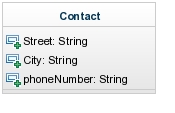
\includegraphics[width=5cm]{figures/exp_contact.jpg}
\caption{Počáteční model}
\label{fig:exp_contact}
\end{center}
\end{figure}

\begin{figure}[H]
\begin{center}
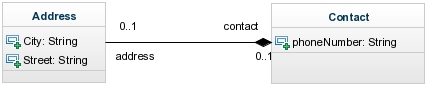
\includegraphics[width=12cm]{figures/exp_contact_address.jpg}
\caption{Cílový model}
\label{fig:exp_contact_address}
\end{center}
\end{figure}

\FloatBarrier

Algoritmus předpokládá, že operace přibližující aktuální stav k cílovému by
měly být rozpoznány (a aplikovány) co nejdříve. Například pro počáteční model
zobrazený na obrázku \ref{fig:exp_contact} a cílový model zobrazený na obrázku
\ref{fig:exp_contact_address}. 
Pokud použijeme základní definici vzdálenosti energie, můžeme
počáteční model vyjádřit pomocí jednoduché textové formy se
zkrácením názvů na počáteční písmeno a dolním indexem pro
property s neunikátním názvem "$M_1$(Cscp)" a cílový model jako $M_2(Cpc_{on},
Acsa)$ vzdálenost těchto dvou modelů vyjádřit pomocí
 delta notace zobrazené v seznamu \ref{algo:state:delta_example}.
 
\begin{lstlisting}[mathescape,frame=single,caption=Textový patch
modelů pro ukázkový příklad v delta notaci,label=algo:state:delta_example]
   +C$c_{on}$    -Csc
   +A            
   +Asca
\end{lstlisting}


$$distance(M_1,M_2) = E(C_{12}) + E_{P_{12}} + E(C_{12})
+ E_{P_{12}} = 0 + 2 + 1 + 4 = 7$$

Algoritmus v prvním průchodu rozpozná, že je možné aplikovat operace
AddClass, RemoveProperty a ExtractClass. Nejlepším parametrem pro AddClass je
třída Address. AddClass zlepšuje vzdálenost o 1. Nejlepším parametrem pro
operaci RemoveProperty je jedna z odstraněných property, takže například
Street. RemoveProperty zlepšuje vzdálenost také o 1. Vhodnými
parametry pro operaci ExtractClass jsou třídy zdrojová třída Address,
extrahovaná třída Contact, referenční property contact, její oppositum address a
nějaký seznam properties obsažených v třídě address.
Nejlepšími parametry pro ExtractClass jsou dvě zmiňované třídy s asociačními
properties a seznam všech properies v nově vzniklé třídě Contact. ExtractClass
má hodnotu zlepšujícího kroku 7. Z těchto operací vyhodnotí jako nejlepší
ExtractClass a následně algoritmus skončí, protože po aplikaci se současný
model dostal do cílového stavu a již nerozpozná další operaci.


Algoritmus dává stejnou váhu atributům jako třídám, což nemusí být
správné. Aby algoritmus lépe splňoval požadavky uživatele, tj. priorizoval
některé operace, je možné modifikovat výpočet energie a místo konstanty 1 v
předešlých vzorcích použít konfiguraci vah jednotlivých atributů.
Všechny atributy jsou vyjmenovány v seznamu \ref{algo:state:attribute_list}.

\begin{itemize}\label{algo:state:attribute_list}
   \item Váhy atributů třídy
   \begin{description}
      \item[W(classname)] jméno třídy
      \item[W(parent)] reference na rodičovskou třídu 
   \end{description}
   \item Váhy atributů všech property
   \begin{description}
      \item[W(propertyName)] jméno property
      \item[W(type)] reference na typ property
      \item[W(isOrdered)] boolean značící ordered kolekci
      \item[W(isUnique)] boolean značící unikátní kolekci
      \item[W(LowerBound, UpperBound)] horní a dolní mez hodnot property
   \end{description}
   \item Váhy atributů asociačních property
   \begin{description}
      \item[W(oppositteProperty)] reference na opozitní property u bidirectional
      vazby
   \end{description}
\end{itemize}

\ \\
Příklad konfigurace:
\begin{itemize}
      \item W(classname) = 1
      \item W(parent) = 0 
      \item W(propertyName) = 1
      \item W(type) = 0
      \item W(isOrdered) = 0
      \item W(isUnique) = 0
      \item W(LowerBound, UpperBound) = 0
      \item W(oppositteProperty) = 0
\end{itemize}

Tato konfigurace redukuje získávání energie na původně zmiňovaný způsob definice
Energie.

Další možnou modifikací je úprava seznamu $R_{ops}$ použitého v algoritmu na
řádku \ref{algo:state:forOps}.
Algoritmus je schopný rozpoznat jednotlivé operace, ale může mít problémy s rozpoznáním
některých dvojic operací. Problematickým stavem je například, pokud jediným
rozdílem je primitivní typ property odlišný ve vstupním a výstupním modelu.
Algoritmus vyhodnotí vzdálenost > 0 a musí buď aplikovat operaci RemoveProperty,
která smaže property a má záporný zlepšovací krok. Bylo by nutné upravit
zisk zlepšujícího kroku, značně zesložitit implementaci metody getImprovement
pro operaci RemoveParent, upravit inicializaci zlepšujícího kroku tak, aby se
na řádku \ref{algo:state:improvement}
nainicializovala hodnotou $-\infty$ a
upravit terminální condition na řádku \ref{algo:state:terminal_condition}, tak,
aby algoritmus neběžel do nekonečna. Druhou možností vyřešení tohoto problému je
definovat seznam $R_{ops}$ nikoliv jako seznam operací v aplikačním
metamodelu, ale jako seznam sekvencí operací. Konverze původního seznamu operací
na jednoprvkové sekvence a rozšíření seznamu $R_{ops}$ o sekvenci operací
RemoveProperty a AddProperty, s metodou getImprovement získávání zlepšujícího
kroku pouze pro případy, kdy existuje property, která má v výstupním modelu
jiný typ než ve vstupním.

     
Přes počáteční slibné výsledky testované na konstruktivních operacích nebyl
tento algoritmus shledán jako příliš efektivní. První nevýhodou je, že
algoritmus v každém kroku hledá nejlepší zlepšující krok i pro všechny operace nalezené v
iteraci minulé. Rozpoznané operace z minulého kroku by bylo možné zapamatovat,
ale nebyl nalezen způsob hledání konfliktních operací vyjma případů, kdy dvě
operace pracují nad jinou hierarchickou strukturou. Proto se nedá jednoduše
analyzovat, pro které operace je nutné hledat nový zlepšující krok znovu,
kterých operací se aplikace rozpoznané operace nedotkla, a které operace již
nemusí mít zlepšující krok shodný a mohou mít jiné parametry.

Druhou nevýhodou je šířka prohledávaného stromu - algoritmus testuje v každé
iteraci všechny operace, jejichž seznam (či v modifikaci zmiňovaná sekvence
operací) $R_{ops}$ může nabývat velkých hodnot. Při všech váhách nastavených na
jedna při vzdálenosti dvou modelů distance $distance(M_1,M_2) = d$, velikosti
$R_{ops} = n$, složitosti aplikace operací $op_{appply}$, složitosti zisku zlepšujícího kroku operace
$op_{getImprovement}$ a složitosti zisku parametrů $op_{getParams}$
má algoritmus algoritmickou složitost $O(d) = O((Max(op_{getImprovement})^n *
op_{getParams} * op_{appply})^d)$. V každé z maximálně d iterací je nutné v
nejhorším případě získat zlepšující krok pro každou operaci a pro operaci s
nejvyšším zlepšujícím krokem potom nalézt pro tuto operaci nejlepší parametry a
aplikovat ji. Složitost operace $op_{getImprovement}$ se různí v závislosti na
typu operace. Pro c tříd ve vstupním modelu a výstupním modelu má složitost
hledání parametrů operace AddClass $O(AddClass_{getImprovement})= c^2$ a,
protože hledáme třídu, která není ve vstupním modelu, ale je ve výstupním, tedy
procházíme c tříd ve vstupním modelu a c tříd v modelu výstupním. Složitost
$O(ExtractClass_{getImprovement})= c^2 * p * r * p $ příčemž c je počet tříd ve
vstupním a výstupním modelu, p je maximální počet operací ve třídě a r je počet
extrahovaných property. Hledáme třídu, ve které existuje asociační property v
cílovém modelu, která neexistovala v modelu zdrojovém, jejíž součet energie
properties, které jsou "extrahovány" do třídy typu asociace je největší.
Po položení r = p dostáváme $O(ExtractClass_{getImprovement})= c^2 * p^3 $.
Vzhledem k standardním modelům, které obsahují hodně malých tříd můžeme za
předpokladu $c >> p$ položit $O(op_{getImprovement})= c^2$. U většiny
operací hledáme třídu ze vstupního modelu, ke které hledáme její protějšek ve
výstupním modelu se zadanými vlastnostmi, proto berme $O(op_{getImprovement})= c^2$. Stejnou
složitost získáme ekvivalentním postupem pro funkci getParams.
Funkce $op_{appply})^d)$ hledá jen třídu z vstupního modelu, na které
provede nějaké změny, takže můžeme aproximovat její algoritmickou složitost
hodnotou c.

$O((Max(op_{getImprovement})^n * op_{getParams} * op_{appply})^d) = O(c^2 * c^2
* c)^d = O(c^{5*d})$

Stavový algoritmus měl definován krok pro operace AddPrimitiveClass,
AddStandardClass, RenameEntity, RemoveEntity, RenameProperty.
 
 \section{Návrh ze studia článků}
 
 Kvůli přílišné obecnosti algoritmů pro graph matching nebyly tyto algoritmy
 shledány za vhodné k použití pro problém hledání sady aplikačních operací.
 První 3 popsané algoritmy model matchingu ( 1 párování podle statického
 identifikátoru, 2. signature based matching, 3.
 similarity based matching) nejsou vhodné k použití z důdodu, že k rozpoznání
 popsaných expanzivních a reduktivních operací je nutné rozpoznat 2 třídy,
 které se mapují na jednu třídu pro reduktivní operace a naopak jednu operaci,
 která se mapuje na 2 třídy. Problém rozpoznávání operací je tudíž nadskupinou
 problému model matchingu, protože matching páruje 1 ku 1, ale algoritmus řešící
 problém rozpoznávání operací musí řešit matching M entit
 ku N entitám.
 
 Zmiňované algoritmy mě inspirovaly k vytvoření Custom language specific
 matching algoritmu pro tento problém, který si z zmiňovaných algoritmů v
 sekci \ref{model_matching_principles} bere hlavně poznámku u algoritmu UMLDiff
 zmiňovaného pod Custom Language skupinou \ref{UML_Diff} - ze všech praktických důvodů
 považujeme třídy se stejným jménem jako shodné.

 Vznikly dvě implementace párovacích algoritmů. 
 
 \section{Základní párovací algoritmus}
 První, jednodušší implementace používá základu z UMLDiffu a očekává, že dvě
 třídy se stejným jménem jsou shodné, páruje tedy třídy podle jména, podobně
 předpokládá, že dvě property ve stejné tříde se stejným jménem jsou shodné.
 Následné rozdíly řeší rozpoznáním konstruktivních a destruktivních, případně
 některých operací modifikačních, ať už tyto operace pracovali s třídami nebo s
 property.
 
 Základní algoritmus pracuje podle pseudokódu \ref{algo:matching}

 \begin{algorithm}
 \caption{Základní párovací algoritmus}\label{algo:matching}

\begin{algorithmic}[1]
   \Require Zdrojový model S, cílový model T
   \Ensure Seznam operací $R_{ops}$, po jejichž aplikaci se model S transformuje
       na model T
   \Statex
   \State \textbf{Inicializace:}
   \State $SClses \gets S.classes$ \Comment{Nespárované třídy z vstupního
      modelu} 
   \State $TClses \gets T.classes$ \Comment{Nespárované třídy z
      cílového modelu}
   \State $SProps \gets S.classes.properties$ \Comment{Nespárované properties
      z vstupního modelu}
   \State $TProps \gets T.classes.properties$ \Comment{Nespárované properties
      z cílového modelu}
   \State $R_{ops} \gets \{\}$
   \Statex	   
   \State MATCH\_CLS\_BY\_NAME()
   \State $R_{ops}$= RECOGNIZE\_OPS()\Comment{Rozpoznání operací}
   \State \textbf{END\_ALGORITHM}
   \Statex
   \Procedure{match\_cls\_by\_name}{}
   \ForAll{$C_S \in S.classes$} \label{algo:matching:forEqualCls}
      \ForAll{$C_T \in T.classes$}
         \If{$C_T.name = C_S.name$}
   	        %\State markMatched(S, T, 'Equal') \Comment{Vytvoření equal páru}
   	        \State MATCH\_EQUAL\_PROPS(S, T) \Comment{Aktualizace nespárovaných
   	        properties}
   	        \State $SClses \gets SClses \setminus \{ C_S\}$
   	        \Comment{Aktualnizace nenamatchovaných tříd ze zdrojového modelu}
   	        \State $TClses \gets TClses \setminus \{ C_T\}$\Comment{Aktualizace
   	        nenamatchovaných tříd z cílového modelu}   	        
   	     \EndIf
      \EndFor
   \EndFor
  \EndProcedure	      
   \Statex	
   \Procedure{match\_equal\_props}{clsSrcModel, clsTargetModel)}
   	   \ForAll{$P_S \in clsSrcModel.properties$}
   	      \ForAll{$P_T \in clsTargetModel.properties$}
   	        \If{$P_S.name = P_T.name$}
   	           %\State markMatched($P_S, P_T$, 'Equal')
   	           \State $SProps \gets SProps \setminus \{ P_S\}$
   	           \State $TProps \gets TProps \setminus \{ P_T\}$
   	        \EndIf
   	      \EndFor
   	   \EndFor
   \EndProcedure  
\end{algorithmic}
\end{algorithm}
\FloatBarrier

Algoritmus inicializuje množiny nespárovaných tříd z vstupního (a výstupního)
modelu všemi třídami z vstupního (resp výstupního modelu) a seznam výstupních
operací prázdnou množinou. Následně algoritmus zpáruje třídy podle jména,
odstraní spárované třídy z množin SClasses a TClasses a zpáruje jejich property
podle jména v proceduře MATCH\_EQUAL\_PROPERTIES. Procedura
MATCH\_EQUAL\_PROPERTIES odstraní property ze spárovaných tříd se shodným jménem
z množin SProps a TProps.

Algoritmus pokračuje rozpoznáváním operací. V fázi rozpoznávání operací jsou
již spárovány všechny třídy, které základní párovací algoritmus dokáže
rozpoznat. 

Základní algoritmus rozpoznává operace v pořadí takovém, aby zajistil nejdříve
existenci správné třídy pro přesouvané a odstraňované properties.
Následně algoritmus modifikuje třídy modifikačními operacemi. Tato úprava musí
být provedena před prací s properties, protože algoritmus v některých
modifikačních operacích upravuje množiny SProps a TProps. Následně algoritmus
upraví properties modifikačními operacemi pro properties, aby dostal
properties do cílového stavu nebo do stavu, kdy je možné je z modelu
odstranit. Po úpravě properties odstraní přebytečné properties obsažené v
kolekci SProps. V posledním kroku algoritmus smaže odstraněné třídy. Tento
základní proces je zobrazen na aktivity diagramu \ref{fig:recog_ops_order1}.
Diagram má téměř lineární formu a rozpoznání jednotlivých skupin operací má
tedy pro základní algoritmus v zásadě jednoznačné pořadí.

\begin{figure}[H]
\begin{center}
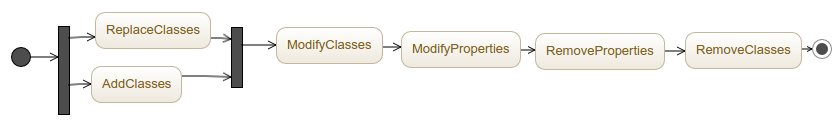
\includegraphics[width=15cm]{figures/recognition_order_basic1.jpg}
\caption{Rozpoznávání operací pořadí}
\label{fig:recog_ops_order1}
\end{center}
\end{figure}


Základní párovací algoritmus dělí třídy do tří skupin:
\begin{enumerate}
   \item třídy, které byly v průběhu Evoluce modelu zachovány
   \item třídy, které byly v průběhu Evoluce z modelu odstraněny
   \item třídy, které byly v průběhu Evoluce do modelu přidány
\end{enumerate}

Základní algoritmus předpokládá, že s třídami z první skupiny bylo manipulováno
pouze za pomoci třídních modifikačních operací a s
properties těchto tříd mohlo být manipulováno pomocí konstruktivních,
destruktivních nebo modifikačních operací. Třídy z druhé skupiny byly z modelu
odstraněny pomocí operace RemoveEntity. Aby byly validační podmínky
destruktivních operací platné, je nutné před aplikací destruktivních operací
RemoveEntity odstranit přebytečné properties operací RemoveProperty a upravit
třídy pomocí třídních modifikačních operací RemoveParent. Třídy v třetí skupině
je nutné do modelu přidat konstruktivní operací AddClass, následně je možné s
třídami manipulovat pomocí třídních modify operací a modifikovat properties
pomocí konstruktivních, destruktivních a modifikačních operací.
Jediné modifikační třídní operace, které mají vliv na strukturu modelu a byly
zařazeny do rozpoznávání jsou operace AddParent a RemoveParent. Operace
AddParent může v nynější implementaci odstraňovat z aktuálního modelu
kolizní properties, má tedy vliv na seznam nenamapovaných properties SProps a
musí předcházet operaci RemoveProperty. 
\\
\begin{figure}[H]
\begin{center}
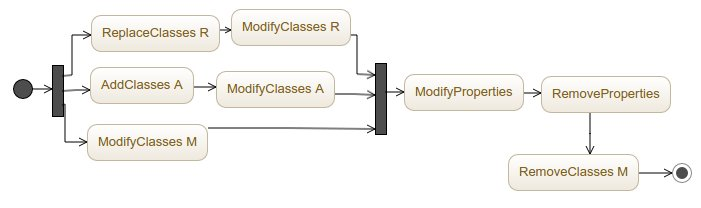
\includegraphics[width=15cm]{figures/recognition_order_basic2.jpg}
\caption{Rozpoznávání operací pořadí, více tříd}
\label{fig:recog_ops_order2}
\end{center}
\end{figure}
\FloatBarrier

 Algoritmus by mohl rozpoznat operace v libovolné přípustné sekvenci. Tato
 přípustná sekvence operací musí splňovat precedenční vztahy zobrazené na obr.
 REF DOPLNěného obr. Každý model je možné rozdělit na množinu nezávislých
 hierarchických strukturálních operací. Dvě třídy A, B patří pro základní
 párovací algoritmus do stejné hierarchické struktury pokud $A.parent = B \vee
 B.parent = A \ \vee \ (\exists X \in M.clses: X \in ancestor(A)\ \wedge\ X \in
 ancestor(B))$, přičemž ancestor(Z) je množina všech předků třídy Z. Sekvence
 operací $op_1, op_2, \ldots op_n$ je nezávislá, pokud všechny operace z
 vstupního modelu operují nad třídami třídami z různých hierarchických struktur
  a žádná z operací op není AddParent. 
  
 Pro každou skupinu množinu operací $\{op_1, op_2, \ldots op_n\}$ můžeme najít
 grupu operací - tj seznam operací operujících nad jedinou hierarchickou
 strukturou či více hierarchickými strukturami spojenými sjednocenými operací
 AddParent.
 
 Nejjednodušší implementací zisku validní sekvence je předpoklad existence
 jediné grupy, tj rozpoznávání operací po skupinách ze seznamu 
 ref algo:match:ops\_seq. Tato implementace je zobrazena v pseudokódu \ref{algo:matching:ops_recognition}
 \\
 Základní rozpoznávací algoritmus má schopnost rozeznat jen konstruktivní,
 destruktivní a modifikační operace. Zachovává data, jejichž identifikátor se
 nemění.
 Ostatní data naopak nekompromisně maže. Tento algoritmus není schopný
 rozpoznat operace RenameClass, RenameProperty, které jsou dle \cite{Luksch}
 nejčastěji používanými operacemi. Tento algoritmus není schopný
 rozpoznat ani žádné expanzivní a reduktivní třídní operace. Výhodou
 implementace tohoto algoritmu je, že nepotřebuje definovat žádný diff
 metamodel. Za předpokladu $C_S \gg P_S \ a\ C_T \gg P_T \ a\  C_S \approx C_T =
 c$ má tento algoritmus složitost $O(c^2)$, protože
 prochází všechny třídy v zdrojovém modelu a hledá pro ně třídu se stejným
 jménem v modelu cílovém.
 
 

\begin{algorithm}
 \caption{Rozpoznání operací v základním
 algoritmu}\label{algo:matching:ops_recognition}

\begin{algorithmic}[1]
   \Statex
   \Procedure{recognize\_ops}{}
   \ForAll{$C \in TClses$}
   \State $ops \gets R_{ops} \bigcup AddCls(C.name)$
   \EndFor
   \Statex
   \ForAll{$C \in TClses$} \Comment{Oprava parency 1.AddParent pro přidané
   Neimplementováno}
      \If{ $C.parent \neq NULL $}
         \State $ops \gets R_{ops} \bigcup AddParent$
         \ForAll{$P \in C.properties and P \in SProps$}
            \State $SProps \gets SProps \setminus P$
         \EndFor
      \EndIf
   \EndFor
   \Statex
   \ForAll{$C \in SClses$} \Comment{Oprava parency 2.
   RemoveParent pro smazané. Neimplementováno}
      \If{ $C.parent \neq NULL $}
         \State $ops \gets R_{ops} \bigcup RemoveParent$
         \ForAll{$P \in C.properties and P \in C.parent.properties$}
            \State $TProps \gets TProps \bigcup P$
         \EndFor
      \EndIf
   \EndFor
   \Statex
   \ForAll{$C_T \in T.Classes \setminus TClses$} \Comment{Oprava parency 3 a 4
   pro namatchované}
      \ForAll{$C_S \in S.Classes \setminus SClses$}
         \If{$C_S.name = C_T.name \wedge C_S.parent = NULL \wedge C_T.parent
         != null$}
            \State $ops \gets R_{ops} \bigcup AddParent$
            \ForAll{$P \in C.properties and P \in SProps$}
               \State $SProps \gets SProps \setminus P$
            \EndFor
         \EndIf
      \EndFor
   \EndFor
   \Statex
   \ForAll{$P \in TProps$}
   \State $ops \gets R_{ops} \bigcup AddProperty(P.owner, P.name)$
   \EndFor
   \Statex
   \ForAll{$P \in SProps$}
   \State $ops \gets R_{ops} \bigcup RemoveProperty(P.owner, P.name)$
   \EndFor
   \Statex
   \ForAll{$C \in SClses$}
   \State $ops \gets R_{ops} \bigcup RemoveCls(C.name)$
   \EndFor   
   \Statex
   \State ADD\_MODIF\_PROP\_OPS()
   \EndProcedure
\end{algorithmic}
\end{algorithm}

\FloatBarrier
 
 \section{Rozšířený algoritmus}
 Složitější implementace algoritmu páruje stejně jako jednodušší v
 první fázi shodné elementy - modely se mění, ale některé třídy jsou zachovány.
 
 Algoritmus předpokládá, že napárované elementy tvoří tzv. páry. Každá třída ze
 zdrojového modelu může být nahrazena, expandována nebo redukována. \\
 
 Třída je nahrazena (tvoří replacing pár), pokud je její jméno změněno či je
 třída zachována. Třída je zachována, pokud v cílovém modelu existuje třída se
 stejným jménem. Algoritmus zavrhuje sekvenci operací mazající všechny
 properties této třídy, smazání třídy a opětovnému vytvoření této třídy s
 jejich properties. Problém hledání RenamePair bude diskutován později. Každá
 třída může být součástí maximálně jednoho replacing páru. Je tedy zakázáno, aby
 v byla třída součástí dvou replacing párů, jednoho replacing a jednoho rename
 páru či dvou rename párů.
 
 Redukované a expandované páry jsou navázány na právě jeden replacing pár.
 
 Třída tvoří redukovaný pár, pokud existuje v zdrojovém modelu, ale neexistuje
 v modelu cílovém a je podobná třídě v cílovém modelu, která je již součástí
 replacing páru.
 
 Třída tvoří expandovaný pár, pokud neexistuje v zdrojovém modelu,
 ale existuje v modelu cílovém a je podobná třídě ze zdrojového modelu, která
 je již součástí replacing páru.\\
 
 Oproti základní verzi algoritmu je nutné vytvořit entitu reprezentující shodu -
 EqualClassPair. Shodné třídy a třídy přejmenované potom tvoří pilíře pro
 operace reduktivní a expanzivní, které se vážou na rozpoznané páry. Operace
 expanzivní a reduktivní není tedy možné bez jejich pilířů rozpoznat. V
 druhé fázi algoritmus páruje již spárované třídy v zdrojovém modelu s třídami
 nespárovanými z cílového modelu a obráceně třídy nespárované ze zdrojového
 modelu s třídami spárovanými. V druhé fázi párování musí algoritmus párovat
 třídy podle jiného kritéria.
 Tímto mnou zvoleným kritériem je suma properties se shodným jménem. Čím vyšší
 je tento koeficient, tím jsou si třídy podobnější.\\
 
 Algoritmus počítá podobnost tříd pomoci počtu properties se stejným jménem.
 Další možností by byla definice energetické funkce viz sekce
 \ref{sec:algo_state}. Aby bylo snazší rozpoznat operace reduktivní a
 expanzivní, byly zavedeny ClassPairy a PropertyPairy.
 
\subsection{Diff elementy}\label{subsect:Diff elementy}
 
 Kvůli nutnosti rozpoznávat operace vznikly v aplikačním metamodelu nové
 elementy. Základní párovací algoritmus si nepotřebuje uchovávat páry,
 třídy jsou spárovány jen na základě shodnosti jména, takže je kdykoliv
 v průběhu algoritmu tento seznam i jednotlivé páry možné získat. Na druhé
 straně rozšířený párovací algoritmus může rozpoznat operaci i RenameEntity a
 její vstupní a výstupní třídu tvořící pár není možné snadno identifikovat.
 Rozšířený párovací algoritmus rozpoznává operace závislé na dvou podobnostech,
 proto je nutné vytvořit 2 páry. První pár určí, která třída byla zachována, či
 měla změněné jméno. Druhý pár potom pomoci podobnosti určí, jestli 
 
  Kořenovým elementem diff modelu je Diff element.
 Tento element obsahuje kolekce elementů classpairs typů ClassPair, propertyPairs
 typu PropertyPair, a dále pak addedClasses a removedClasses typu DiffClass a
 addedProperties a removedProperties typu DiffProperty. Element ClassPair
 shlukuje spárované zdrojové (source) a obrazové (reflection) třídy, dále pak
 referenci owningDiff na Diff element, v kterém jsou obsaženy a která je
 důležitá pro implementaci algoritmu a v neposlední řadě underlyingPairs -
 shodné páry Properties typu EqualPropertyPair, které jsou detekované danou
 operací. Podobně jako operace jsou i páry rozděleny do několika skupin.
 
 Konstruktivní a destruktivní operace nemají svůj obraz v diff metamodelu. Je s
 nimi v rámci rozšířeného algoritmu zacházeno stejně jako v základním párovacím
 algoritmu.
 Konstruktivni ani destruktivní operace nejsou reprezentovány jako ClassPair ani
 PropertyPair, protože tyto operace nemapují element ze vstupního modelu na
 element z výstupního modelu.
 Konstruktivní operace by jinak mapovaly prázdný vstup na element a
 destruktivní obráceně element na prázdný výstup.
 
 Oproti jednodušším konstruktivním a destruktivním operacím jsou operace
 expanzívní a reduktivní a modifikační v Diff modelu zobrazeny jako
 ExpansiveClassPair a ReductiveClassPair, které mapují element
 vstupního modelu na element cílového modelu. 
 
 Aby bylo možné rozpoznat specifický pár závislý na jiném páru je nutné při
 nejd, byla přidána třída ReplacingClassPair - nahrazující pár, který se
 používá jako pivot pro hledání expansivních, reduktivních a modifikačních
 párů. Od elementu ReplacingClassPair dědí elementy EqualClassPair - třída,
 která si uchovala jméno z původního modelu a element ReplacingClassPair -
 reprezentující třídu, která si neuchovala jméno, ale má změněný název.
 Podmínky získávání konkrétních typů párů a jejich pořadí specifikuje konkrétní
 rozpoznávací algoritmus.
 
 Projevem konstruktivních a destruktivních operací jsou elementy DiffClass a
 DiffProperty, které zaobalují třídy a property tak, aby bylo možné referencovat
 na jiný objekt než element Structure. 

\subsection{Popis rozšířeného párovacího algoritmu}
Pseudokód rozšířeného algoritmu je zobrazen na \ref{algo:matching_ext}

Algoritmus potřebuje kromě vstupních dat přenesených z původního algoritmu i
počet matchovacích fází, které budou v rámci podobnosti provedeny.

V inicializační fázi stejně jako základní párovací algoritmus nainicializuje
množiny nespárovaných tříd SClses a TClses, množiny nespárovaných properties
SProps a TProps a seznam rozpoznaných operací $R_{ops}$.
Oproti základnímu algoritmu musí nainicializovat i množinu spárovaných tříd
CPairs a množinu spárovaných properties PrPairs. Párem p properties je
uspořádaná dvojice $(P_S, P_T)$ , kde $P_S$ je property ze zdrojového modelu
a $P_T$ je property z modelu cílového, třídě $P_S$ v páru p. Navzdory názvu pár
naznačujícího dvojici elementů, je CPair uspořádaná čtveřice $(C_S, C_T, Pairs,
owningPair)$, kde $C_S$ je třída ze vstupního modelu, $C_T$ je třída z cílového
modelu, třídě $C_S$ v páru říkejme zdrojová třída, třídě $C_T$ potom obrazová třída.
Pairs je množina párů, které náleží danému spárování, dá se říci, že Pairs je množina
párů podobnosti signalizující spárování tříd, která je využita v dalších fázích
algoritmu. OwningPair je nepovinná složka - představuje referenci na
ReplacingPair u Reduktivních a Expanzivních párů a je použita v dalších fázích
algoritmu. Základní párovací algoritmus nepotřeboval zaznamenávat páry, protože
sprárované třídy byly jednoznačně identifikovány svým názvem.

V základní kostře algoritmu se rozšířená verze párovacího algoritmu příliš
neliší od základní verze.  Algoritmus po inicializaci provede párování tříd
podle jména a párování tříd podle podobnosti a zakončí svůj běh rozpoznáním
operací.

V fázi matchování tříd podle jména jsou třídy ze zdrojového modelu párovány s
třídami z cílového modelu na základě společného jména. Oproti fázi matchování v
základním algoritmu zobrazeném na \ref{algo:matching} je v fázi párování podle
jména nutné vytvořit pár tříd - viz řádek \ref{algo:matching_ext:make_pair}.
Následuje rozpoznání shodných properties v proceduře MATCH\_EQUAL\_PROPS viz.
řádek \ref{algo:matching_ext:match_equal_props}. V této proceduře jsou oproti
základnímu algoritmu vytvořeny shodné páry properties. Shodné páry jsou přidány
do čtveřice Cpair, s nastaveným owningPairem NULL.
% do

Pseudokód \ref{algo:matching_ext:match_similarity} ukazuje průběh párovací fáze
za pomoci podobnosti. V prvním jejím kroku je nainicializován seznam
kandidátů podobnosti pro každou třídu. Třída $C_T$ je podobná třídě zdrojové
třídě $C_S$, pokud existuje nejméně jedna property ve třídě $C_S$, která má
shodné jméno jako property v třídě $C_T$. Množinu podobné tříd nazývejme
množinu kandidátů k párování. Mohou nastat 4 situace pro zdrojovou třídu $C_S$ a
jejího kandidáta k párování $C_T$.

\begin{enumerate}
  \item Pro zdrojovou třídu již existuje replacingPair,pro kandidáta podobnosti
     nikoliv.V tomto případě se algoritmus pokusí vytvořit expanzivní pár
     vytvářející novou třídu viz řádek \ref{algo:matching_ext:expansive_pair}
     v pseudokódu \ref{algo:matching_ext:match_similarity}
  \item Pro zdrojovou třídu $C_S$ i pro jejího kandidáta $C_T$ existuje
     replacingPair viz řádek \ref{algo:matching_ext:modifying operation}
     v pseudokódu \ref{algo:matching_ext:match_similarity}. Tato situace
     zahrnuje jednak spárování tříd v rámci replacing páru a také oddělené
     spárování v rámci modifying operací.
  \item Pro zdrojovou třídu neexistuje replacingPair, ale pro kandidáta
     podobnosti existuje replacing pár. viz řádek
     \ref{algo:matching_ext:reductive_pair} v pseudokódu
     \ref{algo:matching_ext:match_similarity}. V této situaci se algoritmus
     pokusí spárovat třídy do reductivního páru. 
  \item Pro zdrojovou třídu ani pro kandidáta podobnosti neexistuje
     replacingPair. viz řádek \ref{algo:matching_ext:rename_pair} v
     pseudokódu \ref{algo:matching_ext:match_similarity}. V této situaci se algoritmus
     pokusí spárovat třídy do RenamePáru páru. Tato situace může zakrývat
     situaci 1 či 3
\end{enumerate}

Aby byla třída spárována do reduktivního nebo expanzívního páru, musí být
splněny podmínky vycházející z aplikace dané reduktivní či expanzivní operace.

 Pro ilustraci si představme, že máme zdrojový model $M_1 = (Abcde)$ a cílový
 model $M_2 = (Abcf, Bdeg)$. Diff těchto dvou modelů je zobrazen na výpisu
 \ref{algo:match_ext:delta_exp}

 \begin{lstlisting}[frame=single,caption=Textový diff pro
 expanzivní operaci,label=algo:match_ext:delta_exp]
   +B            -Ade
   +Bdeg          
   +Af
\end{lstlisting}
 
 Vidíme, že třída A byla zachována, třída B, třída B je podobná A s koeficientem
 podobnosti 2, existují 2 property("e" a "d") ve třídě A ve zdrojovém modelu se
 shodným jménem jako mají property v modelu cílovém ve třídě B. Třída B byla
 přidána do modelu a je podobná třídě A, algoritmus očekává rozpoznání
 expanzivní operace. Pokud je přidaná property "f" typu B a property "g" ve
 třídě B je typu A, algoritmus rozpozná operaci ExtractClass. Pokud v
 cílovém modelu platí B.parent = A, algoritmus rozpozná operaci ExtractSubClass.
 V případě nerozpoznaného typu páru algoritmus skončí s matchovací fází, protože
 neexistuje jiný kandidát pro třídu B na vytvoření páru a podobnost bude
 zanedbána.\\
 
 V ilustračním příkladě 2 zaměníme $M_1$
 za model $M_2$ v původním příkladu, tj. $M_2 = (Abcde)$ a $M_1 = (Abcf,
 Bdeg)$. Textový diff je zobrazen na výpisu \ref{algo:match_ext:delta_red}
 
  \begin{lstlisting}[frame=single,caption=Textový diff pro
 reduktivní operaci,label=algo:match_ext:delta_red]
   +Ade          -B            
                 -Bdeg          
                 -Af
\end{lstlisting}
 
 Algoritmus pro tento příklad zjistí, že třída A byla zachována, třída B byla
 odstraněna, z třídy B byly odstraněny properties "d", "e" a "g", z třídy A
 byla odstraněna property f, naopak do třídy A byly přidány property "de". Třída
 B je podobná s koeficientem 2 (shodnost properties "d" a "e") třídě A. Třída B
 byla ze zdrojového modelu odstraněna, algoritmus prověřuje reduktivní operace.
 Pokud platí B.parent = A algoritmus rozpozná operaci CollapseHierarchy, v
 případě, že property f a g tvoří oboustraně navigabilní vazbu, algoritmus
 rozpozná operaci InlineClass. V případě, že algoritmus nerozpozná ani jeden z
 těchto párů bude podobnost zanedbána.

\begin{algorithm}
 \caption{Rozšířený párovací
 algoritmus}\label{algo:matching_ext}

\begin{algorithmic}[1]
   \Require Zdrojový model S, cílový model T, C počet matchovacích fází
   \Ensure Seznam operací $R_{ops}$, po jejichž aplikaci se model S transformuje
       na model T
   \Statex
   \State \textbf{Inicializace:}
   \State $SClses \gets S.classes$ \Comment{Nenamatchované třídy z vstupního
      modelu} 
   \State $TClses \gets T.classes$ \Comment{Nenamatchované třídy z
      cílového modelu}
   \State $SProps \gets S.classes.properties$ \Comment{Nenamatchované properties
      ze vstupního modelu}
   \State $TProps \gets T.classes.properties$ \Comment{Nenamatchované properties
      z cílového modelu}
   \State $R_{ops} \gets \{\}$
   \State $CPairs \gets \{\}$
   \State $PrPairs \gets \{\}$
   \Statex	   
   \State MATCH\_CLSES\_BY\_NAME()
   \State MATCH\_CLSES\_BY\_SIMILARITY(C)
   \State $R_{ops}$= RECOGNIZE\_OPS()\Comment{Rozpoznání operací}
   \State \textbf{END\_ALGORITHM}
   \Statex
   \Procedure{match\_clses\_by\_name}{}
   \ForAll{$C_S \in S.classes$} \label{algo:matching:forEqualCls}
      \ForAll{$C_T \in T.classes$}
         \If{$C_T.name = C_S.name$}
   	        \State cPair = markMatched(S, T, 'Equal') \Comment{Vytvoření equal
   	        páru}
   	        \label{algo:matching_ext:make_pair} 
   	        \State  pairs = MATCH\_EQUAL\_PROPS(S, T)
   	        \State  addUnderlyingPairs(cPair, pairs)
   	        \State  $CPairs = CPairs\ \bigcup \ cPair$
   	        \Comment{Aktualizace nespárovaných properties}
   	        \State $SClses \gets SClses \setminus \{ C_S\}$
   	        \Comment{Aktualnizace nenamatchovaných tříd ze zdrojového modelu}
   	        \State $TClses \gets TClses \setminus \{ C_T\}$\Comment{Aktualizace
   	        nenamatchovaných tříd z cílového modelu}   	        
   	     \EndIf
      \EndFor
   \EndFor
  \EndProcedure	      
   \Statex	
   \Procedure{match\_equal\_props}{clsSrcModel, clsTargetModel)}
   \label{algo:matching_ext:match_equal_props} \State Pairs = \{\}
   	   \ForAll{$P_S \in clsSrcModel.properties$}
   	      \ForAll{$P_T \in clsTargetModel.properties$}
   	        \If{$P_S.name = P_T.name$}
   	           \State pair = markMatched($P_S, P_T$, 'Equal')
   	           \State $Pairs = Pairs\ \bigcup\ pair$
   	           \State $SProps \gets SProps \setminus \{ P_S\}$
   	           \State $TProps \gets TProps \setminus \{ P_T\}$
   	        \EndIf
   	      \EndFor
   	   \EndFor
   	   \State \textbf{return } Pairs
   \EndProcedure  
\end{algorithmic}
\end{algorithm}

\FloatBarrier
 
\begin{algorithm}
 \caption{Matchování podle podobnosti rozšířeného
 algoritmu}\label{algo:matching_ext:match_similarity}
 \begin{algorithmic}[1]
 \Procedure{match\_clses\_by\_similarity}{iterCount}
    \State CSets = initSimilarityCandidates() \Comment {mapa kandidátů CSets}
    \For{i = 0 ; i < iterCount ; i++}\Comment{Proveď iterCount párovacích
    iterací}
       \ForAll{$cls \in CSets.keys()$}
          \State candidates = CSets.get(cls)
          \State $MATCH\_CLS\_BY\_SIMILARITY(cls, candidates)$
       \EndFor
    \EndFor
 \EndProcedure
 \Statex
 \Procedure{match\_cls\_by\_similarity}{sourceCls, reflectionCandidates}
 	\ForAll{$candidate \in reflectionCandidates$}
 	   \If{isReflectionReplacingPairRecognised(candidate)}
 	      \If{isSourceClassReplacingPairRecognised(sourceCls)}
 	         \State \Comment{Nevzniká nový pár, je rozpoznána modifying operace
 	         ve fázi rozpoznávání operací}\label{algo:matching_ext:modifying
 	         operation}
 	      \Else
 	         \State matchReductivePair(sourceCls, candidate)
 	         \label{algo:matching_ext:reductive_pair}
 	      \EndIf
 	   \Else
 	      \If{isSourceClassReplacingPairRecognised(sourceCls)}
 	         \State matchExpansivePair(sourceCls,
 	         candidate)\label{algo:matching_ext:expansive_pair}
 	      \Else
 	         \State matchRenamePair(sourceCls,
 	         candidate)\label{algo:matching_ext:rename_pair}
 	      \EndIf
 	   \EndIf 
 	\EndFor
 \EndProcedure
 \end{algorithmic}
\end{algorithm}

\FloatBarrier

% *****************************************************************************

\chapter{Testování projektu Migdb}\label{chapt:testování}

V průběhu vývoje byl za účelem ověření správné funkcionality vytvořen projekt
Migdb.testing.run, který spouští jednotlivé testy kompoment aplikace. 

V rámci projektu byly vytvořeny testy komponent Workflow obsažené v packagi
migdb.testing.components.run, testy aplikační evoluce inkludované do Workflow
test\_app\_atomic.mwe2 v packagi migdb.testing.app.atomic.run, testy databázové
evoluce obsažené workflow test\_rdb\_atomic.mwe2 v packagi
migdb.testing.rdb.atomic.run, testy validátorů aplikačního a databázového
modelu obsažené v packagi migdb.testing.validators.run, test ORM transformace
struktury aplikace na DB schema + ORMo transformace obsažené v workflow
migdb.testing.orm.run, testy generování SQL schématu obsažené v packagi
migdb.testing.generators.run, integrované testy celého frameworku migdb
obsažené v packagi migdb.testing.migdb\_executer a posledními testy jsou testy
algoritmů rozpoznávajících operace obsažené v packagi
migdb.testing.app.oracle.run.

Testy komponent testují správnou funkcionalitu komponenty Comparator, která
musí správně porovnat očekávaný a reálný výstupní soubor xmi ostatních testů.
Tyto testy jsou rozděleny do více workflow, protože některé musí být neúspěšné,
jak už napovídá klíčové slovo fail v jejich názvu. Dalšími komponentami
vzniklými v rámci projektu Migdb byly QVTOExecutor, TestWorkflow,
DirectoryCleaner a TestComponent. Komponenta TestComponent vznikla, aby bylo
přehlednější a efektivnější psát QVT testy Migdb, je složena z několika dalších
načítacích, ukládacích a porovnávacích komponent a zkracuje zápis testů ve
workflow asi 10 krát. Nebylo jasné, jak vytvořit testy na správnou funkcionalitu
ostatních komponent - správné jejich zapojení do jiných testů bylo pro nás
dostatečným testem.

Ostatní testy se řadí do xmi kategorie testů, tj testů, které mají jako
vstupní model xmi soubor. Po spuštění xmi testů se v projektu
migdb.testing.run vygeneruje složka output-tests, která obsahuje výstupní data 
jednotlivých testů. Výstupní data mohou obsahovat výstupní xmi soubory
porovnávané s očekávaným xmi souborem nebo SQL souborem, který je možné
aplikovat na databázi PostgreSql.

Speciálním testem je test\_code\_generator.mwe2, tento test vygeneruje pro
zadaný vstupní aplikační model a sadu aplikačních operací výstupní rdb model, sadu
databázových operací, výstupní SQL generující strukturu databáze a SQL
reprezentující výstupní databázové operace. Kromě těchto vygenerovaných dat je
možné najít ke každému testu v adresáři test\_data reálná data, s kterými může
být test spuštěn. Reálná data jsou vytvořena jen pro testy komplexnějších
operací (operace 007 - 010), které jen nemění strukturu databáze, ale i
manipulují s daty. Postup testování tohoto testu je - spuštění workflow vedoucí k
vygenerování SQL db schematu a SQL db operací. Spuštění SQL vytvářející
strukturu databáze, spuštění SQL s daty uloženými v souboru data.sql z
přidružené složky v adresáři test\_data, aplikace vygenerovaného souboru
transformačních SQL, zobrazení výstupních dat za pomoci souboru
check\_selects.sql ze složky s daty. Bohužel nebyl nalezen lepší způsob
otestování než manuální spuštění a vizuální porovnáných selectů s očekávaným
výstupem po apliaci dané operace na data.sql.

\chapter{Ukázka zdrojového kódu práce}\label{chapt:ukazka_kodu}


%*****************************************************************************

\chapter{Závěr}\label{chapt:zaver}
Po několikaletém teoretickém a praktickém studiu změn v aplikačním modelu a
jejich projevu v modelu aplikačním se nám podařilo definovat ucelenou množinu
operací, pomocí nichž je možné měnit aplikační model a definovat jejich mapování
na operace databázové úrovně.

Nejjednodušším a teoreticky nejzajímavějším tématem našeho projektu je aplikační
model, kterému byly věnovány celkově 2 bakalářké a 2 diplomové práce
BP - \cite{Tarant_bp} a  \cite{Lukes}, DP \cite{Tarant_dip},  a \cite{Mazanec}.

Implementačně nejnáročnějším a zároveň nejvíce teoreticky vyčerpaným tématem se
stala samotná transformace aplikačních operací na operace databázové, čehož jsem
využil a k implementaci, otestování a dospecifikaci tohoto mapování jsem přidal
téma čerstvé a velmi málo prozkoumané. Tímto atraktivním tématem vzhledem k
verzování modelů je automatické rozpoznávání operací provedených nad aplikačním
modelem.

Mrzí mně, že jsem se nemohl více věnovat tématu rozpoznávání operací nad
aplikačním modelem, takže jsem se nedostal k tématům jako je sémantickém
rozpoznávání operací vycházející pravděpodobně z idei sémantického
webu a implementací Resource Description Framework (RDF) a Ontology Web
Language (OWL). Implementace sémantického rozpoznávání by mohla v budoucnu
odhadnout změny nejen na základě syntaxe(struktury) databáze, ale i na základě
významu názvů jednotlivých entit v databázi. Předpokládám, že potom by bylo
možné detekovat mnohem jednoznačněji přejmenování entit - pokud by pomocí nějaké
ontologie či podobného nástroje bylo jasně specifikováno, že zvíře je nadtypem
býložravce a tento je nadtypem entity zebra, potom pokud v původním modelu
existuje třída Zebra, která má jako rodičovskou třídu nastavenu třídu
Býložravec a v výsledném modelu existuje třída Zebra s nadtřídou Zvíře a
neexistuje třída Býložravec, potom by algoritmus měl snadněji detekovat
přejmenování třídy Býložravec na třídu Zvíře i přes velkou strukturální
podobnost s jinou třídou.

Je otázkou, jak by sémantičtější rozpoznávání operací bylo prospěšné v
kontextu stále větších informačních systémech, kdy je občas těžké nazvat
smysluplně entity aplikačního modelu, natož sémantiku jejich relace vůči jiným
entitám.

V průběhu psaní této diplomové práce jsem si uvědomil, proč pro nás bylo občas
obtížné definovat správné mapování aplikačních operací na operace databázové.
Čím blíže bylo zaměření daného participanta bližší aplikačnímu modelu, tím více
si tento participant přibližoval databázový model aplikačnímu a vznikaly tak
entity jako jsou HasNoInstance s názvem rodičovské tabulky bez jakékoliv relace
rodičovství existující v databázovém modelu. Druhou chybou, kterou jsme
dělali při zaměření se na aplikační metamodel bylo modelování aplikačních
operací, které měly přespříliš složité mapování na databázové operace či někdy
až nesmyslný vliv na data v modelu - příkladem bylo modelování operace
SetOpposite, která v aplikačním modelu spojí dvě existující property tříd a až
při implementaci mapování na databázové operace bylo zjišťěno, že tato operace
pozbývá smyslu. Tato odlehlost členů Migdb od databázového modelu vytvořila
nemalé koncepční problémy, jejichž řešení bylo nutné s nemalým úsilím vymyslet
a implementovat ve velmi pozdní fázi projektu. Pokud bych psal Migdb znovu od
začátku, zaměřil bych se více na kooperaci jednotlivých částí, aby bylo pro mně
psaní transformace ORMo snazší. Tato transformace je esenciální pro chod
projektu a proto je její správná implementace alfa omegou na úspěch projektu.

Samotná definice operací aplikovatelných na databázový model není pevná, což
vzhledem k malému vzorku sbíraných požadavků vede k nejednoznačným ORMo
mapováním. Proto v navazujících pracích by bylo dobré udělat operační výzkum a
získat větší množství požadavků na tyto operace.

Věcí, kterou bych udělal znovu jinak při psaní Migdb od začátku by bylo využití
jiného jazyka než je QVT. Tento mapovací jazyk se našim potřebám hodil málo,
proto jsme časem přestali používat jeho zakladní koncept - mapování a nahradili
ho Java-like programovacím stylem queries a helperů. Naráželi jsme na stále
větší problémy a QVT nám nepřinášelo moc užitku, nýbrž některé nevýhody. Jedna z
těchto nevýhod je například automatické ukládání jakýchkoliv pomocných entit do
výstupních modelů, které bylo nutné vyřešit (za účelem správného
otestování) speciální transformací kopírující jen ty části výstupního modelu,
které byly opravdovým výstupem, nikoliv meziproduktem. Tato transformace
vzhledem ke svojí povaze samozřejmě zpomaluje exekuci Migdb Workflow.

Poslední otázkou, na kterou jsem neměl moc času hledat odpověď je portabilita
projektu Migdb funkčního nad relační databází PostgreSQL na jiné
relační databáze. Předpokládám, že by nebylo složité změnit generátor kódu
pro jiné relační databáze - algoritmus vygenerování SQL kódu je poměrně
přímočarý a pro PostgreSQL nebyl dlouhý. Struktura jiných relačních databází
není vždy stejná, ale většinově se shoduje, takže ani modifikace databázového
metamodelu by neměla být obtížná. Moje minimální zkoumání tohoto tématu
odhalilo, že námi používaná databáze PostgreSQL má maximální délku 64 znaků, 
databáze Oracle má maximální délku identifikátoru 30 znaků a databáze Microsoft 
SQL server má maximum stanoveno na 128 znaků. Z tohoto vyplývá, že převod Migdb 
na databázi Microsoft SQL server by nebyl  z tohoto pohledu problematický.
30 znaků pro Oracle nevypadá jako problematické - vývojáři mají málokdy třídy
ukládané do databáze s jmény delšími než 30 znaků, problém nastává při zahrnutí
service pro získávání názvů databázových entit k entitám z aplikačního modelu.
Získání názvu cizího klíče, kolekce a asociační tabulky spojuje název atributu a
tabulky s nějakým prefixem a odděluje tyto položky jména podtržítky. 

Tudíž skutečné omezení délky názvu třídy může být základních 30 oslabeno o 3
(prefix FK či kolekce), oslabeno o 3 (podtržítka oddělující jednotlivé tři
části jména - prefix a dvě tabulky) děleno 2 (dvě části). Aplikací těchto
operací dostaneme horní hranici 12 znaků, která vypadá jako dostatečná, ačkoliv 
ne tolik komfortní. V této hranici jsme nicméně nezapočítaly Camel-podtržítkovou
konverzi velkých písmen na malá předražená podtržítky. Předpokládejme, že každý
identifikátor nebude mít víc jak 3 slova, tudíž musíme odečíst další 3 znaky. 9
nemusí být vždy dostatečná hranice vzhledem k velikosti nynějších systémů a
nezapočítáváme do toho fakt, že třídy v aplikačním modelu mohou(a často jsou)
prefixovány nějakým workspacem či balíčkem. Tudíž délka 9 nemusí být maximální
horní hranice jmen našich tříd a property. Je tedy zřejmé, že potom bude muset
uživatel projektu Migdb nad databází Oracle používat krátké a naprosto
neintuitivní názvy entit typu Vec102 či je nutné vymyslet jiný způsob překládání
jmen do databázového modelu, který bude automatizovaný, jednoznačný, nezávislý
na ostatních entitách v modelu a nejlépe pro člověka snadno získatelný bez
pomoci nějakého překladače.

Není možné generovat zkrátit názvy entit - vedlo by to u kolizních názvů pomocí
indexace, protože bez dalších pravidel jako například očív případě potřeby
odstranit Constraint není možné zjistit, ke které entitě

%\section{Další poznámky}
%\subsection{České uvozovky}
%V souboru \verb|k336_thesis_macros.tex| je příkaz \verb|\uv{}| pro sázení
% českých uvozovek. \uv{Text uzavřený do českých uvozovek.}

% JZ: 3.5.2009 \chapter z book zajistí automaticky
%\subsection{Začátky kapitol na liché stránky}
%Ve výsledném textu je dobré, když každá kapitola začíná na liché stránce. Tedy použijte:
%\begin{verbatim}
%  \cleardoublepage\include{1_uvod}
%  \cleardoublepage\include{2_teorie}
%   atd.\ldots{}
%\end{verbatim}

%*****************************************************************************
\chapter{Seznam použitých zkratek}\label{chapt:seznam_zkratek}

\begin{description}
\item[IDE] Integrated Development Environment
\item[ORM] Object-relational mapping
\item[EMF] Eclipse modeling framework
\item[SŘBD] Systém řízení báze dat
\item[IO] Integritní omezení
\item[LCS] Longest common Subsequence
\item[OMG] Object Management Group
\item[ORMo] Object-relation mapping of operations
\item[QVT]  Query view transformational
\item[QVTo] QVT operational
\item[DDL] Data definition Language
\item[SŘBD] Systém řízení báze dat
\item[OCL] Object Constraint Language
\end{description}

%*****************************************************************************
%\chapter{UML diagramy}
%\textbf{\large Tato příloha není povinná a zřejmě se neobjeví v každé práci.
% Máte-li ale větší množství podobných diagramů popisujících systém, není nutné všechny umísťovat do hlavního textu, zvláště pokud by to snižovalo jeho čitelnost.}

%*****************************************************************************
\chapter{Instalační a uživatelská příručka}\label{chapt:manual}
\textbf{\large Tato příloha velmi žádoucí zejména u softwarových implementačních prací.}

%*****************************************************************************
\chapter{Obsah přiloženého CD}\label{chapt:obsah_cd}
\textbf{\large Tato příloha je povinná pro každou práci. Každá práce musí totiž obsahovat přiložené CD. Viz dále.}

Může vypadat například takto. Váš seznam samozřejmě bude odpovídat typu vaší práce. 

\begin{figure}[H]
\begin{center}
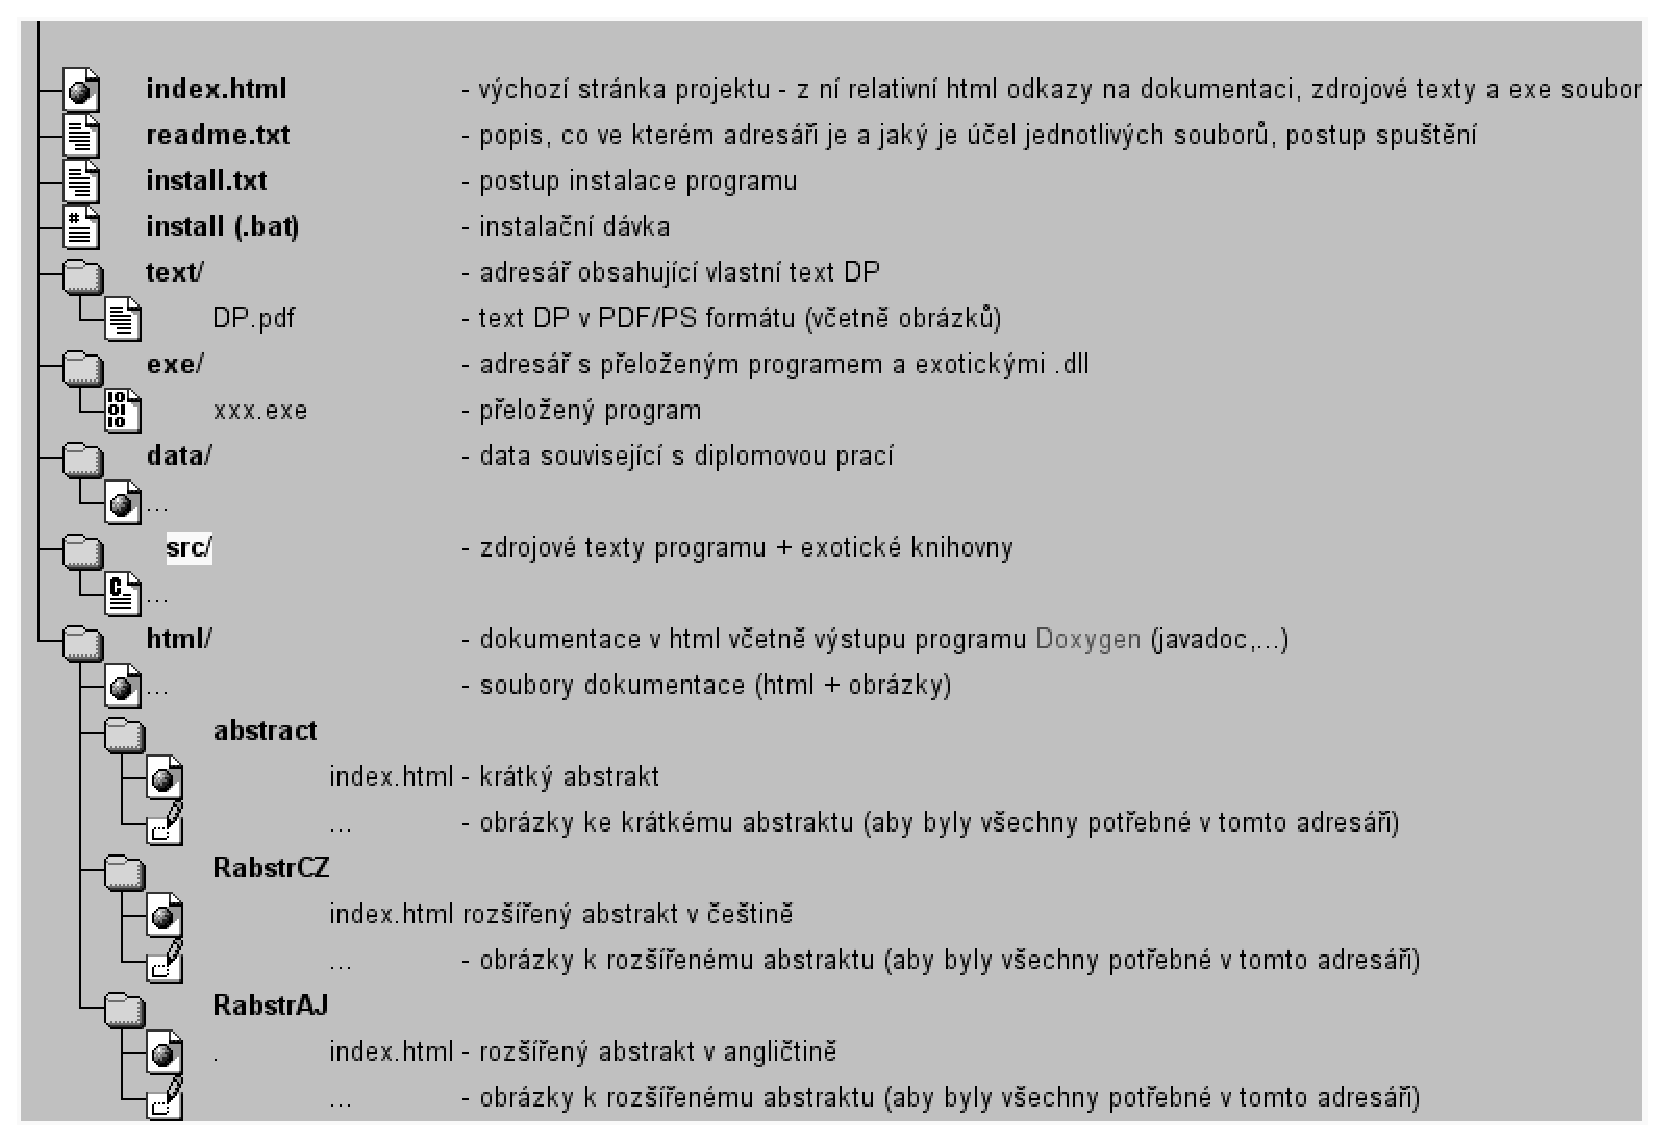
\includegraphics[width=14cm]{figures/seznamcd}
\caption{Seznam přiloženého CD --- příklad}
\label{fig:seznamcd}
\end{center}
\end{figure}

Na GNU/Linuxu si strukturu přiloženého CD můžete snadno vyrobit příkazem:\\ 
\verb|$ tree . >tree.txt|\\
Ve vzniklém souboru pak stačí pouze doplnit komentáře.

Z \textbf{README.TXT} (případne index.html apod.)  musí být rovněž zřejmé, jak programy instalovat, spouštět a jaké požadavky mají tyto programy na hardware.

Adresář \textbf{text}  musí obsahovat soubor s vlastním textem práce v PDF nebo PS formátu, který bude později použit pro prezentaci diplomové práce na WWW.
 \bibliographystyle{alpha}
\bibliography{reference}

\end{document}
